\documentclass[12pt,a4paper]{article}
\usepackage[utf8]{inputenc}
\usepackage[T1]{fontenc}
\usepackage[ngerman]{babel}
\usepackage{graphicx}
\usepackage{geometry}
\geometry{a4paper, margin=1in}
\usepackage{fancyhdr}
\usepackage{hyperref}
\usepackage{listings}
\usepackage{color}
\usepackage{titlesec}
\usepackage{float}
\usepackage{url}
\usepackage{hyperref}
\usepackage{xcolor}


\setcounter{secnumdepth}{7}

\definecolor{dkgreen}{rgb}{0,0.6,0}
\definecolor{gray}{rgb}{0.5,0.5,0.5}
\definecolor{mauve}{rgb}{0.58,0,0.82}

\lstset{
  frame=tb,
  language=Java,
  aboveskip=3mm,
  belowskip=3mm,
  showstringspaces=false,
  columns=flexible,
  basicstyle={\small\ttfamily},
  numbers=none,
  numberstyle=\tiny\color{gray},
  keywordstyle=\color{blue},
  commentstyle=\color{dkgreen},
  stringstyle=\color{mauve},
  breaklines=true,
  breakatwhitespace=true,
  tabsize=3
}

\pagestyle{fancy}
\fancyhf{}
\cfoot{\thepage}

\title{Gesamtprojektdokumentation: Selbstfahrendes Golfcar}
\author{6B Engineering UG (haftungsbeschränkt)\\Dein Name}
\date{\today}

\begin{document}

\begin{titlepage}
    \centering
    \vspace*{1cm}
    
\includegraphics[width=0.5\textwidth]{Resources/company_logo.jpg}\par\vspace{1cm}
    {\LARGE\bfseries Gesamtprojektdokumentation: Selbstfahrendes Golfcar \par}
    \vspace{1.5cm}
    {\Large 6B Engineering\par}
    \vspace{1cm}
    {\large \today \par}
    \vfill
\end{titlepage}

\newpage
\tableofcontents

\newpage
\section{Einleitung}
Die Vision selbstfahrender Fahrzeuge hat in den letzten Jahren erhebliche Aufmerksamkeit in der Technologie- und Automobilbranche erlangt. Unser Projekt nimmt eine einzigartige Stellung in diesem innovativen Feld ein, indem es sich auf die Entwicklung eines selbstfahrenden Autos konzentriert, das speziell für die Aufgabe entworfen wurde, Golfbälle aufzuspüren und einzusammeln. Diese Website dient als zentrale Informationsquelle über unser Projekt, bietet Einblicke in die technischen Spezifikationen, die Teammitglieder und den Entwicklungsprozess. Zudem stellt sie Downloads zur Verfügung, erklärt die verwendeten Bauteile und ermöglicht die Steuerung des Fahrzeugs, das sowohl autonom als auch manuell bedient werden kann, inklusive einer Liveansicht seiner Operationen.

Das Kernziel unseres Projekts ist die Schaffung eines selbstnavigierenden Fahrzeugs, das effizient Hindernisse erkennt und den kürzesten Weg zu seinem Ziel findet, um Golfbälle aufzusammeln. Die Herausforderung besteht darin, präzise Sensoren und fortschrittliche Algorithmen zu integrieren, um eine zuverlässige Funktion unter verschiedensten Bedingungen zu gewährleisten. Unser Ansatz umfasst die Entwicklung eines Miniatur-Golfcars, ausgestattet mit einem innovativen Greifarm, der die Bälle nicht nur lokalisiert und aufnimmt, sondern sie auch präzise in einem dafür vorgesehenen Behälter platziert. Diese Webseite dokumentiert unseren Fortschritt, teilt wichtige Erkenntnisse und dient als Plattform zur Demonstration der vielseitigen Einsatzmöglichkeiten unseres selbstfahrenden Miniatur-Golfcars.


\section{Projektübersicht}
Die Entwicklung des selbstfahrenden Golfcars ist ein ambitioniertes Projekt, das von 6B Engineering UG initiiert wurde, um innovative Lösungen im Bereich der autonomen Fahrzeuge zu erforschen und zu demonstrieren. Dieses Projekt kombiniert fortschrittliche Technologien aus den Bereichen Robotik, maschinelles Lernen und mechanisches Design, um ein Fahrzeug zu entwickeln, das fähig ist, Golfbälle selbstständig zu lokalisieren, aufzusammeln und zu transportieren.

\subsection{Projektziele}
Die Hauptziele des Projekts umfassen:
\begin{itemize}
  \item Entwicklung eines voll funktionsfähigen Prototyps eines selbstfahrenden Golfcars, das in der Lage ist, autonom auf einem Golfplatz zu operieren.
  \item Integration von Sensortechnologien zur Hinderniserkennung und -navigation.
  \item Erstellung einer benutzerfreundlichen Schnittstelle zur Überwachung und Steuerung des Fahrzeugs über eine dedizierte Website.
  \item Förderung der technischen Bildung und Inspiration für zukünftige Ingenieure durch offenen Zugang zu Projektressourcen und Dokumentationen.
\end{itemize}

\newpage

\subsection{Projektkomponenten}
Das Projekt gliedert sich in mehrere Schlüsselkomponenten:
\begin{itemize}
  \item \textbf{Fahrzeugdesign und -konstruktion:} Entwurf und 3D-Druck eines maßstabsgetreuen Modells des Cybertrucks, angepasst an die technischen Komponenten wie Raspberry Pi, Sensoren und Antriebseinheiten.
  \item \textbf{Softwareentwicklung:} Programmierung der Steuerungslogik, einschließlich Algorithmen für autonomes Fahren und maschinelles Lernen zur Objekterkennung.
  \item \textbf{Website-Entwicklung und -Hosting:} Aufbau einer Plattform zur Interaktion mit dem Fahrzeug und zur Bereitstellung von Projektinformationen und Updates.
\end{itemize}

\subsection{Erwartete Ergebnisse}
Das Projekt ist darauf ausgerichtet, am 09. Mai 2024 im Rahmen einer Schulveranstaltung präsentiert zu werden. Die erwarteten Ergebnisse umfassen:

\begin{itemize}
  \item \textbf{Demonstration des Prototyps:} Vorstellung des voll funktionsfähigen Prototyps des selbstfahrenden Golfcars, das die Fähigkeit demonstriert, autonom Golfbälle zu lokalisieren, aufzusammeln und zu transportieren.
  \item \textbf{Dokumentation und Lernressourcen:} Bereitstellung einer umfassenden Dokumentation des Projektverlaufs, der verwendeten Technologien und der Entwicklungsschritte. Diese Dokumentation dient als Lernressource für andere Schüler und Lehrkräfte.
  \item \textbf{Feedback und Weiterentwicklung:} Sammeln von Feedback von Lehrern, Schülern und externen Gästen während der Präsentation, um Verbesserungsvorschläge für zukünftige Iterationen des Projekts zu erhalten.
\end{itemize}

\section{Konstruktion des Autos}
\subsection{Design und Planung}
Die Konstruktion unseres Miniatur-Cybertrucks war durch das ikonische Design des Tesla Cybertrucks inspiriert. Unser Modell wurde im Maßstab 1:17 entworfen, um eine hohe Authentizität zu gewährleisten. Die Planung und das Design erfolgten in Autodesk Inventor, einer fortgeschrittenen CAD-Software, die vor allem auf professionelle Nutzer abzielt. Trotz der anfänglichen Herausforderungen aufgrund der Komplexität der Software, erwies sich die Entscheidung als richtig, da sie es ermöglichte, präzise und detaillierte Modelle zu erstellen, die den Anforderungen unseres Projekts gerecht wurden.

\newpage

\subsection{Anpassung des Chassis}
Das Chassis wurde speziell entworfen, um Komponenten wie Raspberry Pi, ein Breadboard, Motoren, Batterien und Sensoren aufzunehmen. Eine besondere Herausforderung stellte die Platzierung der Ultraschallsensoren dar, da der begrenzte Raum eine optimale Anordnung erschwerte. Durch den Einsatz von Autodesk Inventor konnten wir die Sensoren virtuell positionieren und ihre Ausrichtung so anpassen, dass sie funktional innerhalb des begrenzten Raums operieren konnten.

\subsection{3D-Druck und Komponentenintegration}
Das Chassis wurde extern mittels 3D-Druck in PLA gefertigt, was uns erlaubte, eine präzise und robuste Struktur zu schaffen. Die vorhandenen 3D-Modelle der elektronischen Komponenten wie des Raspberry Pi wurden direkt in das CAD-Modell integriert, was die Konstruktion erheblich vereinfachte. Die Modulbauweise in Autodesk Inventor ermöglichte es uns, das Projekt als Baugruppe zu verwalten, wodurch der gesamte Designprozess modularer und flexibler wurde.

\subsection{Entwicklung des Greifarms}
Der Greifarm, ein zentraler Bestandteil unseres selbstfahrenden Golfcars, wurde entworfen, um Golfbälle aufzunehmen und zu transportieren. Die Konstruktion dieses Mechanismus nutzte einen SG90 Servomotor, der für seine Zuverlässigkeit und Effizienz in Leichtbauanwendungen bekannt ist.

\subsubsection{Konstruktionsprozess}
Die Entwicklung des Greifarms war durch einen iterativen Ansatz geprägt, bei dem mehrere Prototypen in verschiedenen Größen gedruckt wurden, um die optimale Passform für den Golfball zu ermitteln. Dieser Prozess ermöglichte es uns, präzise Anpassungen an den Dimensionen und der Funktionalität des Greifarms vorzunehmen, um eine maximale Effizienz und Zuverlässigkeit zu gewährleisten.

\subsubsection{Material und Montage}
Obwohl die Konstruktion des Greifarms relativ einfach war, erforderte sie präzise Fertigungstechniken, um die gewünschten Ergebnisse zu erzielen. Nachdem die endgültige Version des Greifarms durch 3D-Druck hergestellt wurde, entschieden wir uns für eine einfache, jedoch effektive Befestigungsmethode: Der Arm wurde mit Heißkleber an der Vorderseite des Fahrzeugs fixiert. Trotz der möglicherweise fragwürdigen Wahl dieses Befestigungsmittels erfüllte diese Lösung ihren Zweck ohne Probleme und bestätigte die Funktionalität des Greifarms unter realen Bedingungen.

\begin{figure}[H]
\centering
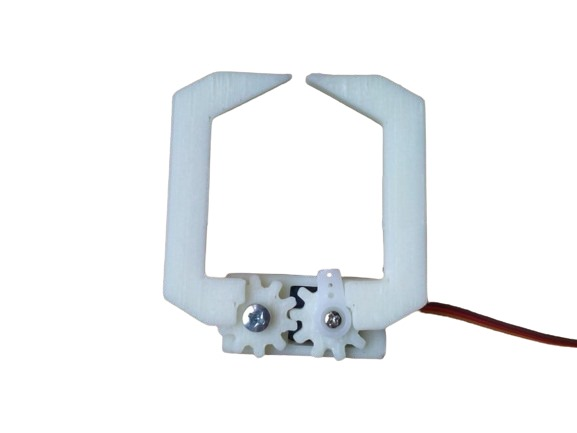
\includegraphics[width=1\textwidth]{Resources/claw_gripper.jpg}
\caption{Der entwickelte Greifarm mit SG90 Servomotor.}
\end{figure}

\subsubsection{Ergebnis und Bewertung}
Die Verwendung des SG90 Servomotors erwies sich als eine ausgezeichnete Wahl für die Steuerung des Greifarms, da er genügend Drehmoment für die Handhabung der Golfbälle bietet, ohne das Gesamtgewicht des Fahrzeugs wesentlich zu erhöhen. Die endgültige Montage, obwohl einfach durchgeführt, zeigte eine robuste Leistung während aller Testphasen und im realen Einsatz auf dem Golfplatz.

\subsection{Problematische Kameraplatzierung}
Ein spezifisches Problem war die Platzierung der Kamera, die wir als "Kameranase" des Fahrzeugs bezeichnen. Die einzige praktikable Lösung, die sich im Rahmen des Designs anbieten ließ, war nicht optimal, da sie Kompromisse in Bezug auf die Sicht und die Ästhetik erforderte. Dennoch war diese Anordnung notwendig, um die Funktionalität des Fahrzeugs in einem realen Umfeld sicherzustellen.

\subsection{Bilder der Konstruktion}
Um einen detaillierten Einblick in die Konstruktionsphase zu geben, zeigen wir hier einige Bilder des Modells aus verschiedenen Perspektiven:

\newpage

\begin{figure}[h]
    \centering
    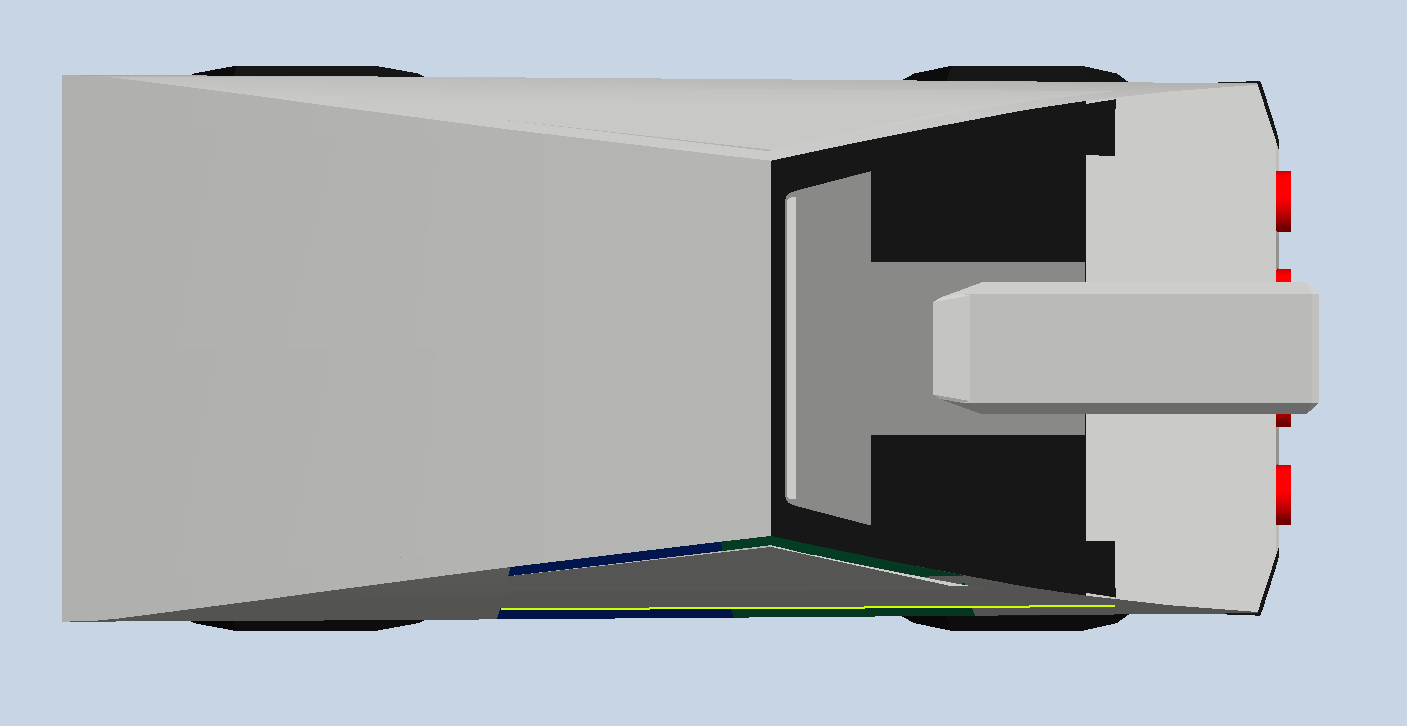
\includegraphics[width=0.95\textwidth]{Resources/oben_normal.png}
    \caption{Ansicht von oben (normal)}
\end{figure}

\begin{figure}[h]
    \centering
    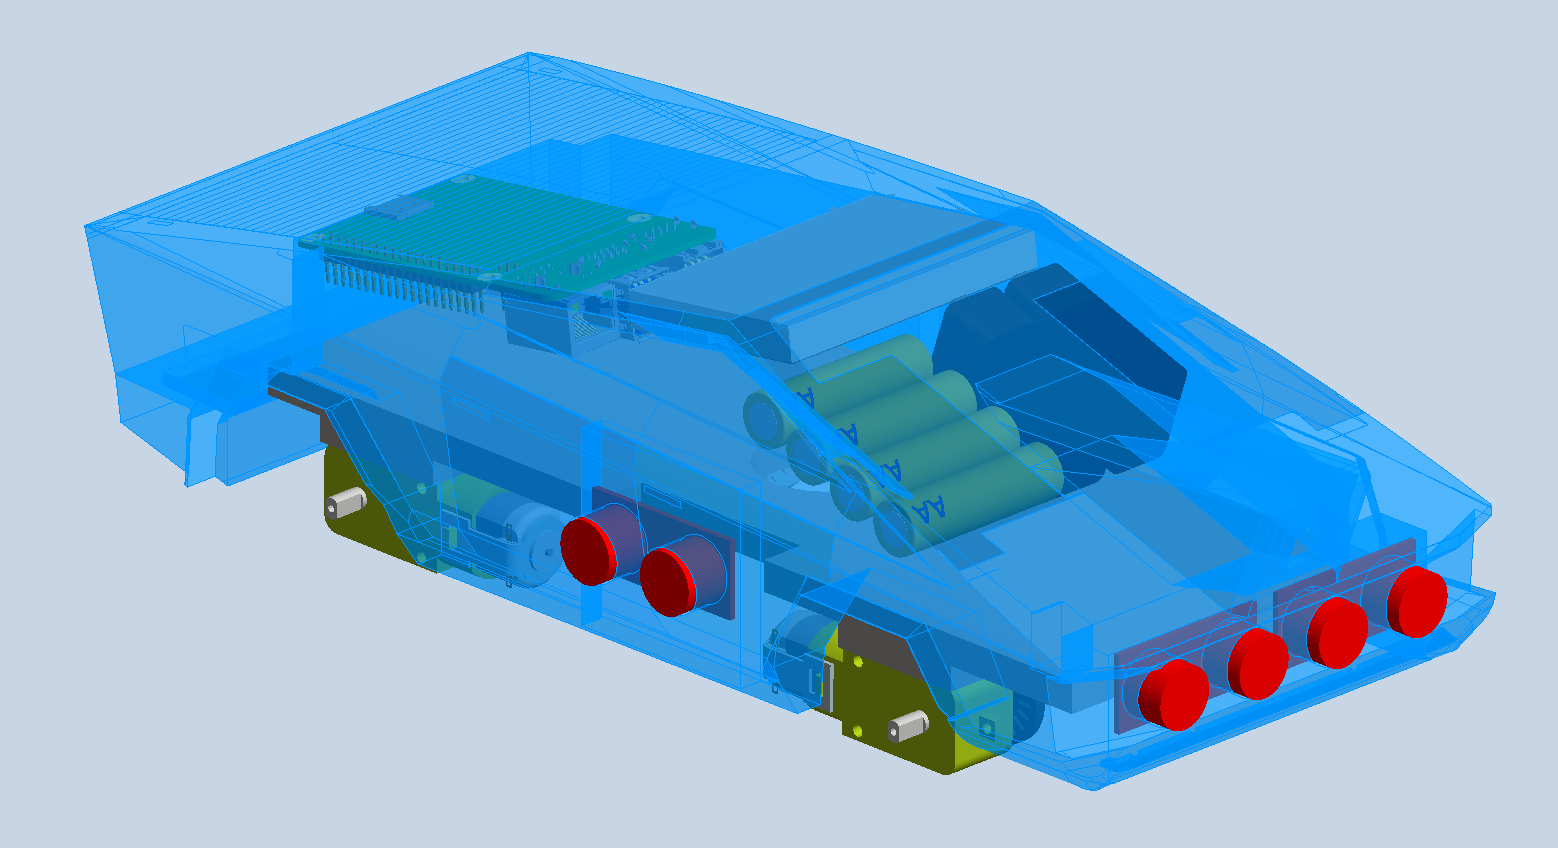
\includegraphics[width=0.95\textwidth]{Resources/seitlich_chassi_transparent.png}
    \caption{Seitenansicht des Chassis (transparent)}
\end{figure}

\newpage

\begin{figure}[h]
    \centering
    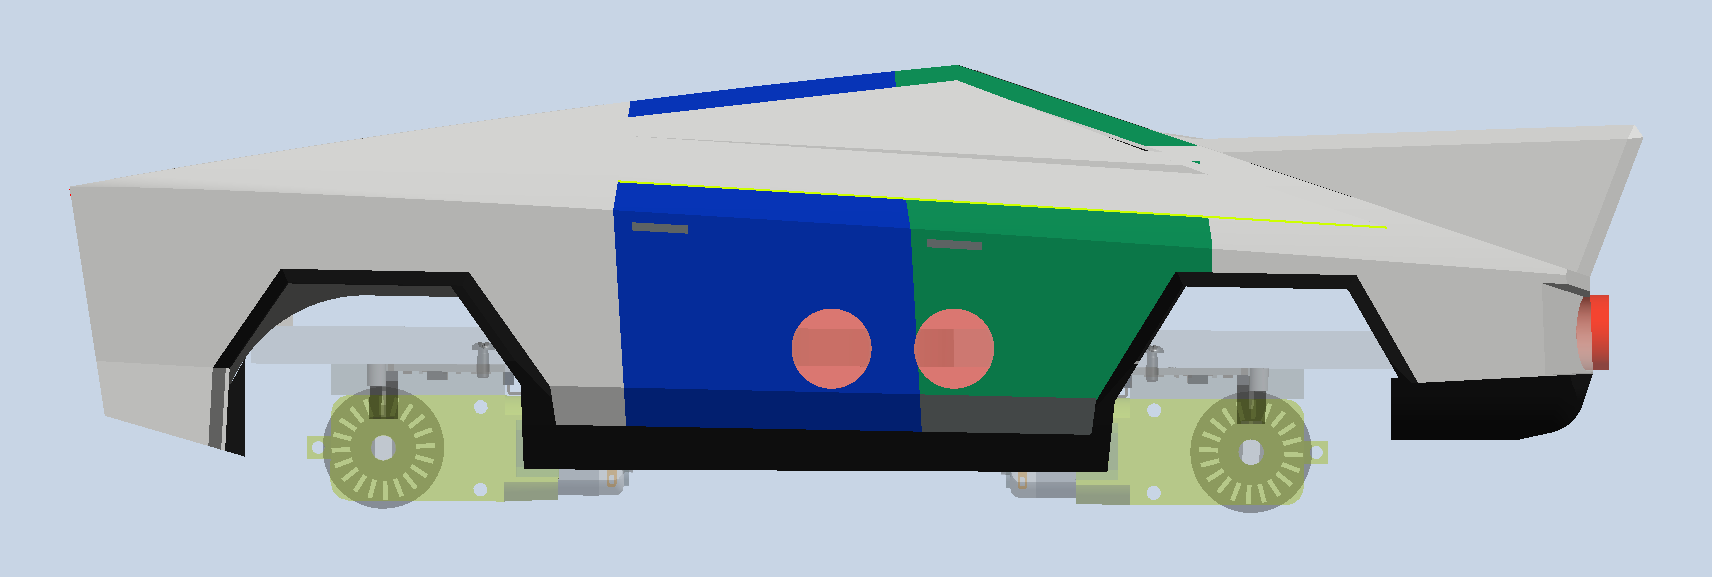
\includegraphics[width=0.99\textwidth]{Resources/seitlich_transparent.png}
    \caption{Seitenansicht (transparent)}
\end{figure}

\begin{figure}[h]
    \centering
    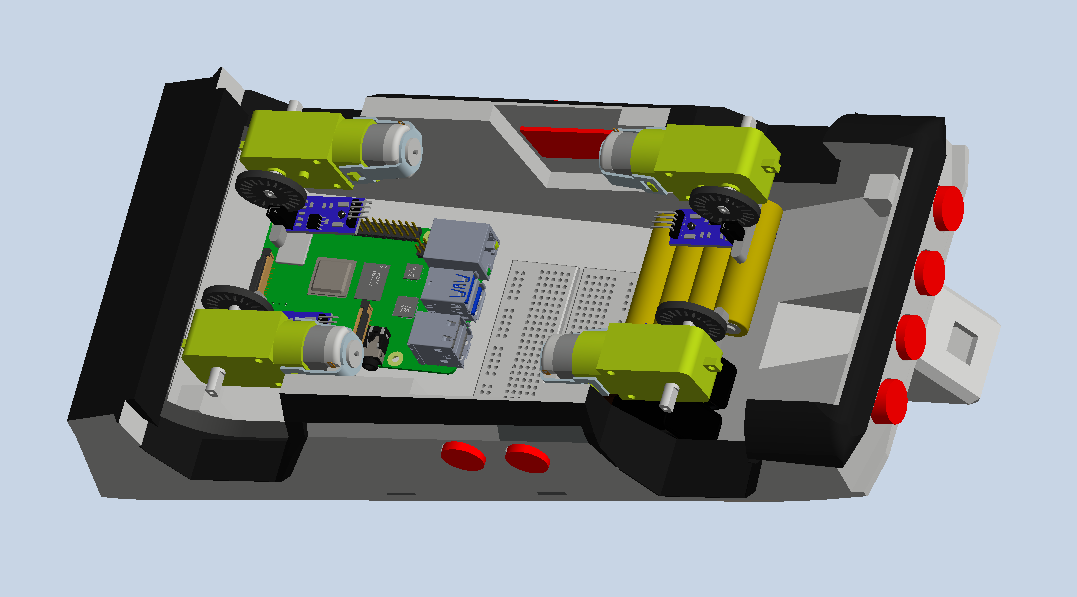
\includegraphics[width=0.99\textwidth]{Resources/unten_ohne_trennplatte.png}
    \caption{Ansicht von unten ohne Trennplatte}
\end{figure}

\newpage

\begin{figure}[h]
    \centering
    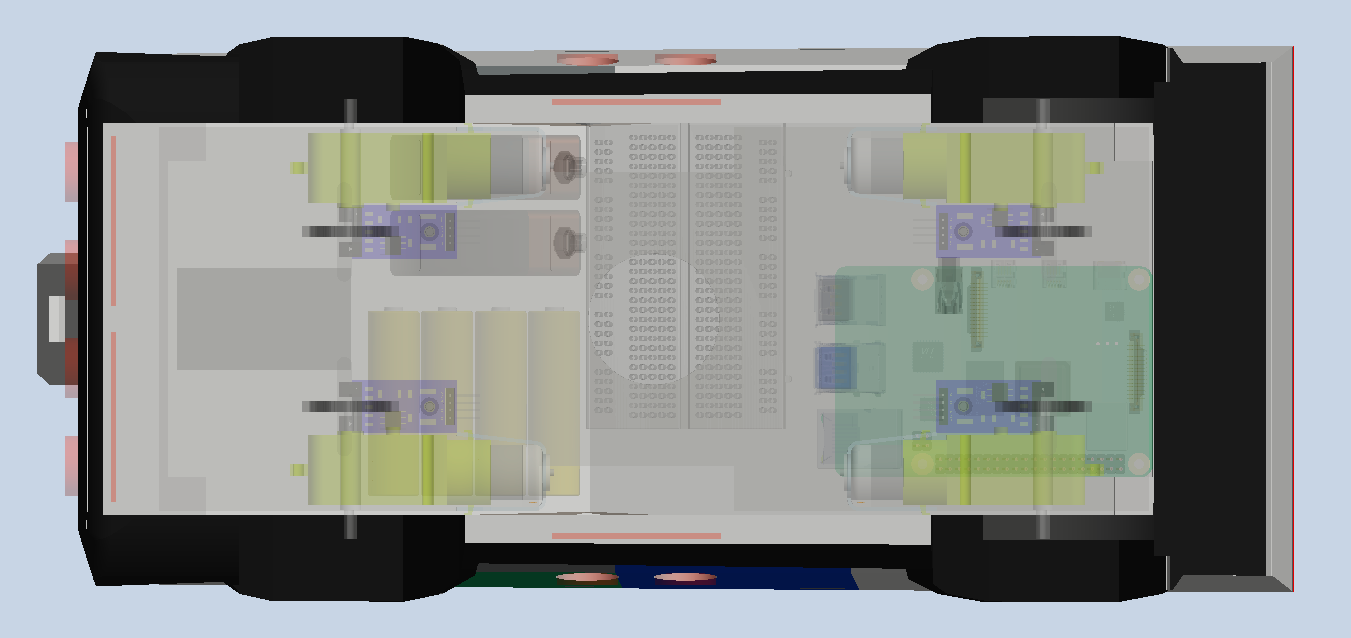
\includegraphics[width=0.95\textwidth]{Resources/unten_transparent.png}
    \caption{Unteransicht (transparent)}
\end{figure}

\begin{figure}[h]
    \centering
    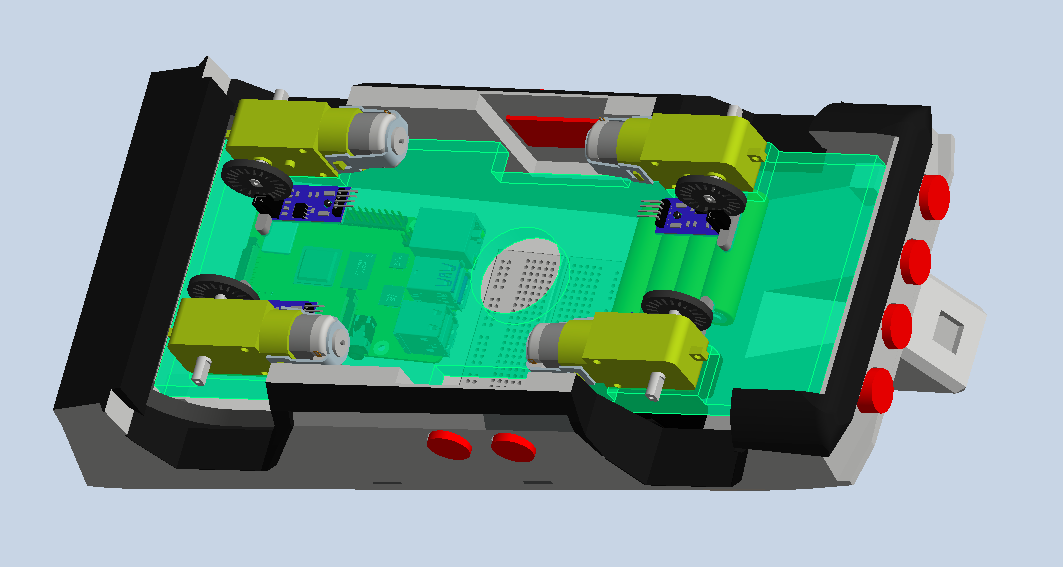
\includegraphics[width=0.95\textwidth]{Resources/unten_trennplatte_transparent.png}
    \caption{Unteransicht mit Trennplatte (transparent)}
\end{figure}

\newpage

\subsubsection{3D-Modellansicht Online}
Um eine interaktive Betrachtung unseres Konstruktionsmodells zu ermöglichen, stellen wir das 3D-Modell über den Autodesk Viewer online zur Verfügung. Dieser Service erlaubt es Nutzern, das Modell in hoher Detailgenauigkeit zu betrachten, ohne spezielle Software installieren zu müssen.

\paragraph{Funktionen des Autodesk Viewers}
Über den folgenden Link können Interessierte das 3D-Modell unseres Miniatur-Cybertrucks in Echtzeit betrachten: \newline \url{https://tinyurl.com/golfcarspace}.
\newline
Mit diesem Tool können Nutzer:

\begin{itemize}
    \item Das Modell aus verschiedenen Winkeln betrachten und um 360 Grad drehen.
    \item In bestimmte Bereiche hinein- und herauszoomen, um spezifische Details zu erkunden.
    \item Verschiedene Ansichten aktivieren, wie transparente Ansichten, um einen Einblick in die interne Platzierung der Komponenten zu erhalten.
    \item Schnittebenen hinzufügen, um Querschnitte des Modells zu analysieren und zu verstehen, wie die einzelnen Teile zusammenpassen.
\end{itemize}

Diese Online-Plattform bietet eine wertvolle Ressource für Kunden und Interessenten, um die technischen Aspekte und die konzeptionelle Gestaltung unseres Projekts tiefgehend zu verstehen. Sie dient nicht nur der Darstellung unseres technologischen Know-hows, sondern ermöglicht auch eine transparente Kommunikation der konstruktiven Leistungen unseres Teams.


\subsection{Schlussfolgerung}
Die Konstruktion unseres Miniatur-Cybertrucks war ein umfangreiches Projekt, das präzise Planung, sorgfältige Ausführung und kreatives Problemlösen erforderte. Die erfolgreiche Umsetzung dieses Teils des Projekts demonstriert unsere Fähigkeit, komplexe technische Herausforderungen zu meistern und innovative Lösungen zu entwickeln.

\newpage


\section{Anwendung von Kanban}
\subsection{Kanban-System}
Um die Organisation und das Management unseres Projekts zu optimieren, implementierten wir ein Kanban-System, das auf einem digitalen Trello-Board von Atlassian basierte. Dieses Tool ermöglichte es unserem Team, den Überblick über alle laufenden Aufgaben zu behalten und den Arbeitsfortschritt effektiv zu verfolgen.

\subsubsection{Kanban-Board-Struktur}
Unser Kanban-Board war in drei Hauptbereiche unterteilt: \textbf{TODO}, \textbf{DOING} und \textbf{DONE}, die uns halfen, den Lebenszyklus jeder Aufgabe von der Planung bis zur Fertigstellung zu visualisieren. 
\begin{itemize}
    \item \textbf{\textcolor{black}{TODO:}} Aufgaben, die geplant und noch nicht begonnen wurden.
    \item \textbf{\textcolor{blue}{DOING:}} Aufgaben, die derzeit in Bearbeitung sind.
    \item \textbf{\textcolor{green}{DONE:}} Aufgaben, die abgeschlossen wurden und keine weiteren Aktionen benötigen.
\end{itemize}

\subsubsection{Farbkodierung}
Zur weiteren Vereinfachung der Übersicht und um unterschiedliche Aspekte des Projekts hervorzuheben, verwendeten wir ein Farbschema für unsere Aufgaben:
\begin{itemize}
    \item \textcolor{blue}{\textbf{Blau}} wurde für die Planungsphasen verwendet.
    \item \textcolor{green}{\textbf{Grün}} stand für Aufgaben, die direkt mit dem Auto zusammenhingen.
    \item \textcolor{red}{\textbf{Rot}} bezeichnete alle Aufgaben, die die Website betrafen.
    \item \textcolor{black}{\textbf{Schwarz}} wurde für Aufgaben verwendet, die die Sensoren des Autos betrafen.
\end{itemize}

\begin{figure}[H]
\centering
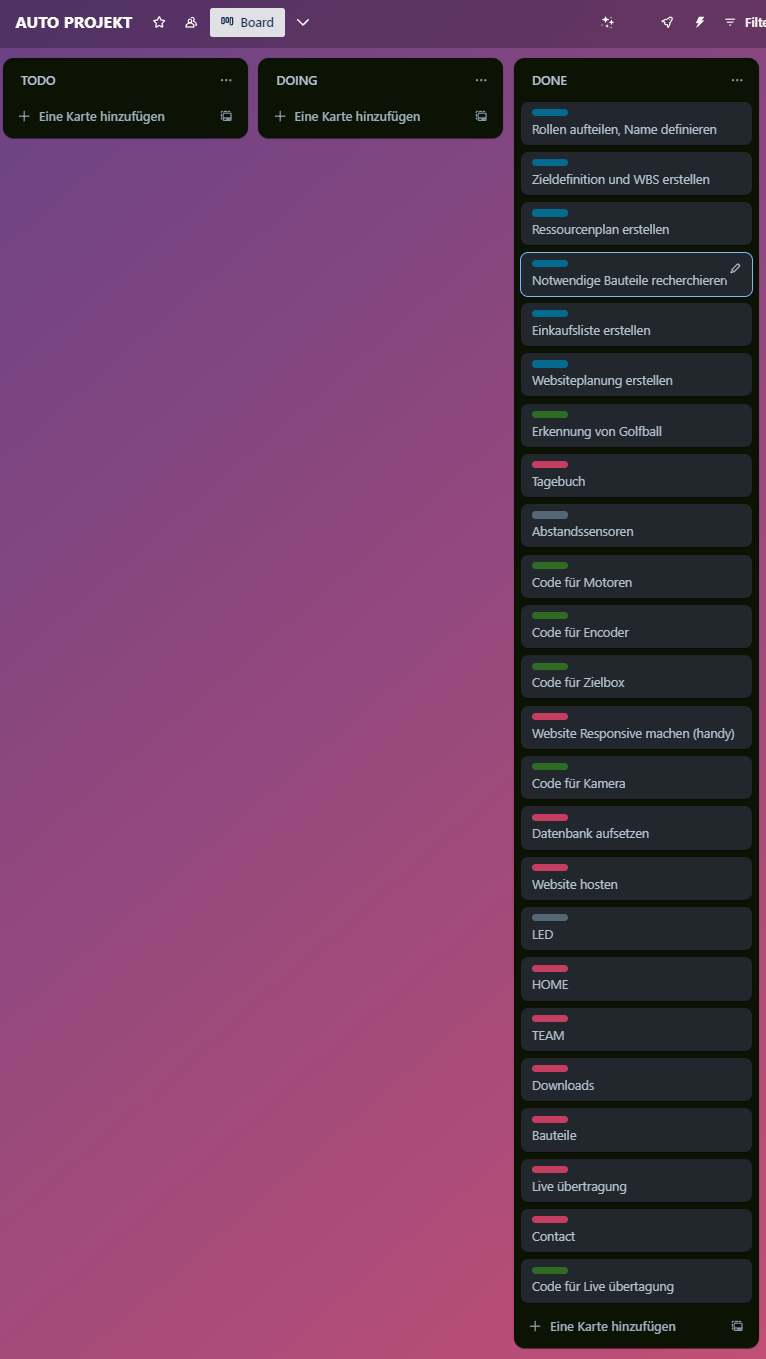
\includegraphics[width=0.85\textwidth]{Resources/kanban_board.png}
\caption{Das Kanban-Board mit farbkodierten Aufgabenbereichen.}
\end{figure}

\subsubsection{Herausforderungen und Vorteile}
Während der Nutzung von Kanban stießen wir auf einige Herausforderungen, insbesondere das gelegentliche Vergessen, Blöcke zu verschieben, was zu zeitweiligen Unklarheiten im Projektstatus führte. Trotz dieser kleinen Schwierigkeiten bot das Kanban-Board einen wertvollen Überblick über den Projektfortschritt und erlaubte es dem Team, effizient zu reagieren und Anpassungen vorzunehmen, wenn nötig.

\subsubsection{Gesamteindruck}
Die Anwendung von Kanban erwies sich als äußerst nützlich, da sie es dem Team ermöglichte, stets einen groben Überblick über den Stand des Projekts zu haben. Diese Methode förderte nicht nur die Transparenz innerhalb des Teams, sondern half auch dabei, die Projektdynamik aufrechtzuerhalten und sicherzustellen, dass alle Aufgabenbereiche angemessen adressiert wurden.


\section{Planung und Projektierung der Website}
\subsection{Einleitung}
Die Website unseres Projekts dient als zentrales Bindeglied zwischen der technologischen Innovation unseres selbstfahrenden Golfcars und der globalen Gemeinschaft von Technikbegeisterten, Bildungseinrichtungen und potenziellen Nutzern. In diesem Abschnitt wird erläutert, wie die Planung und die Umsetzung der Website mit dem Ziel erfolgten, eine benutzerfreundliche, informative und interaktive Plattform zu schaffen. Wir stellen unsere Strategien für das Design, die Benutzerführung und die Inhaltsvermittlung vor und diskutieren, wie diese Elemente dazu beitragen, das Gesamtziel unseres Projekts zu unterstützen. Die Website ist nicht nur eine Darstellung unseres technischen Fortschritts, sondern auch ein Werkzeug, das es ermöglicht, die Fortschritte zu verfolgen, mit dem Team zu interagieren und das Projekt in seiner Entwicklung zu unterstützen.

\subsection{Zielgruppe}
\subsubsection{Hobbybastler}
Das Kernstück unseres Projekts, das selbstfahrende Miniatur-Golfcar, richtet sich an zwei Hauptzielgruppen: Hobbybastler und, in einer späteren Entwicklungsphase, Golfspieler. Hobbybastler stehen im Zentrum unserer Zielgruppe. Durch die Bereitstellung von Bauplänen, Bauteilen und Programmcode auf unserer Website schaffen wir eine Ressource, die es Enthusiasten ermöglicht, tief in die Materie der selbstfahrenden Autos einzutauchen. Unsere detaillierten Dokumentationen und Materialien dienen als Lerngrundlage und Inspirationsquelle für eigene Projekte. Diese Gruppe profitiert insbesondere von der Möglichkeit, die Theorie in die Praxis umzusetzen und durch unsere Anleitungen und Programme eigenständige Fortschritte zu erzielen.

\newpage

\subsubsection{Golfspieler}
In einer zukünftigen Entwicklungsphase zielt unser Projekt darauf ab, auch Golfspieler anzusprechen. Die Vision ist es, ein Fahrzeug zu entwickeln, das auf Golfplätzen autonom verschossene Bälle lokalisieren und einsammeln kann. Dies würde nicht nur die Effizienz auf dem Golfplatz erhöhen, sondern auch ein neues Level an Technologieintegration in den Sport einführen. 

\subsubsection{Bildungseinrichtungen}
Als sekundäre Zielgruppe sehen wir Bildungseinheiten, wie Schulen und Universitäten, die unser Projekt als praktisches Lehrmittel nutzen könnten. Die Vielfalt der technischen Aspekte unseres selbstfahrenden Miniatur-Golfcars bietet eine ausgezeichnete Grundlage für interdisziplinäres Lernen und Experimentieren im Bereich der Robotik, Programmierung und Mechanik.

\subsection{Struktur der Website}

Die Website präsentiert sich mit einer klaren und nutzerzentrierten Struktur, die darauf ausgelegt ist, den Besuchern eine intuitive Bedienung und schnellen Zugriff auf die verschiedenen Sektionen zu ermöglichen.

\subsubsection{Navigationsleiste}
Die Website zeichnet sich durch eine innovative vertikale Navigationsleiste aus, die in der Mitte der Seite angeordnet ist. Bei einem Klick auf einen der Navigationspunkte (\textit{Home}, \textit{About}, \textit{Downloads}, \textit{Bauteile}, \textit{Live}, \textit{Teamspace}) öffnet sich dieser und präsentiert die jeweilige Seite, während die Leiste nach links versetzt wird. Ein erneuter Klick auf den bereits geöffneten Punkt lässt diesen wieder einziehen und zentriert die Navigationsleiste erneut.

\subsubsection{Interaktionselemente}
Die Website bietet verschiedene interaktive Elemente:
\begin{itemize}
    \item Ein \textbf{Live-View-Feature} im Adminbereich, das das Livebild der selbstfahrenden Autos anzeigt.
    \item Downloadbereiche, in denen Besucher alle relevanten Dokumente wie Baupläne, Diagramme und die Codebasis herunterladen können.
    \item Steuerelemente für das Auto, wie Buttons mit Pfeilen für die Richtungssteuerung und einen Start-Button für die automatische Suche.
    \item Ein Kontaktformular, um eine direkte Kommunikation mit dem Team zu ermöglichen.
\end{itemize}

\subsubsection{Usecase-Diagramm}
Ein Usecase-Diagramm wird ergänzt werden, um die Interaktionen der Nutzer mit den verschiedenen Funktionen der Website zu visualisieren. 

\newpage

\begin{figure}[h]
\centering
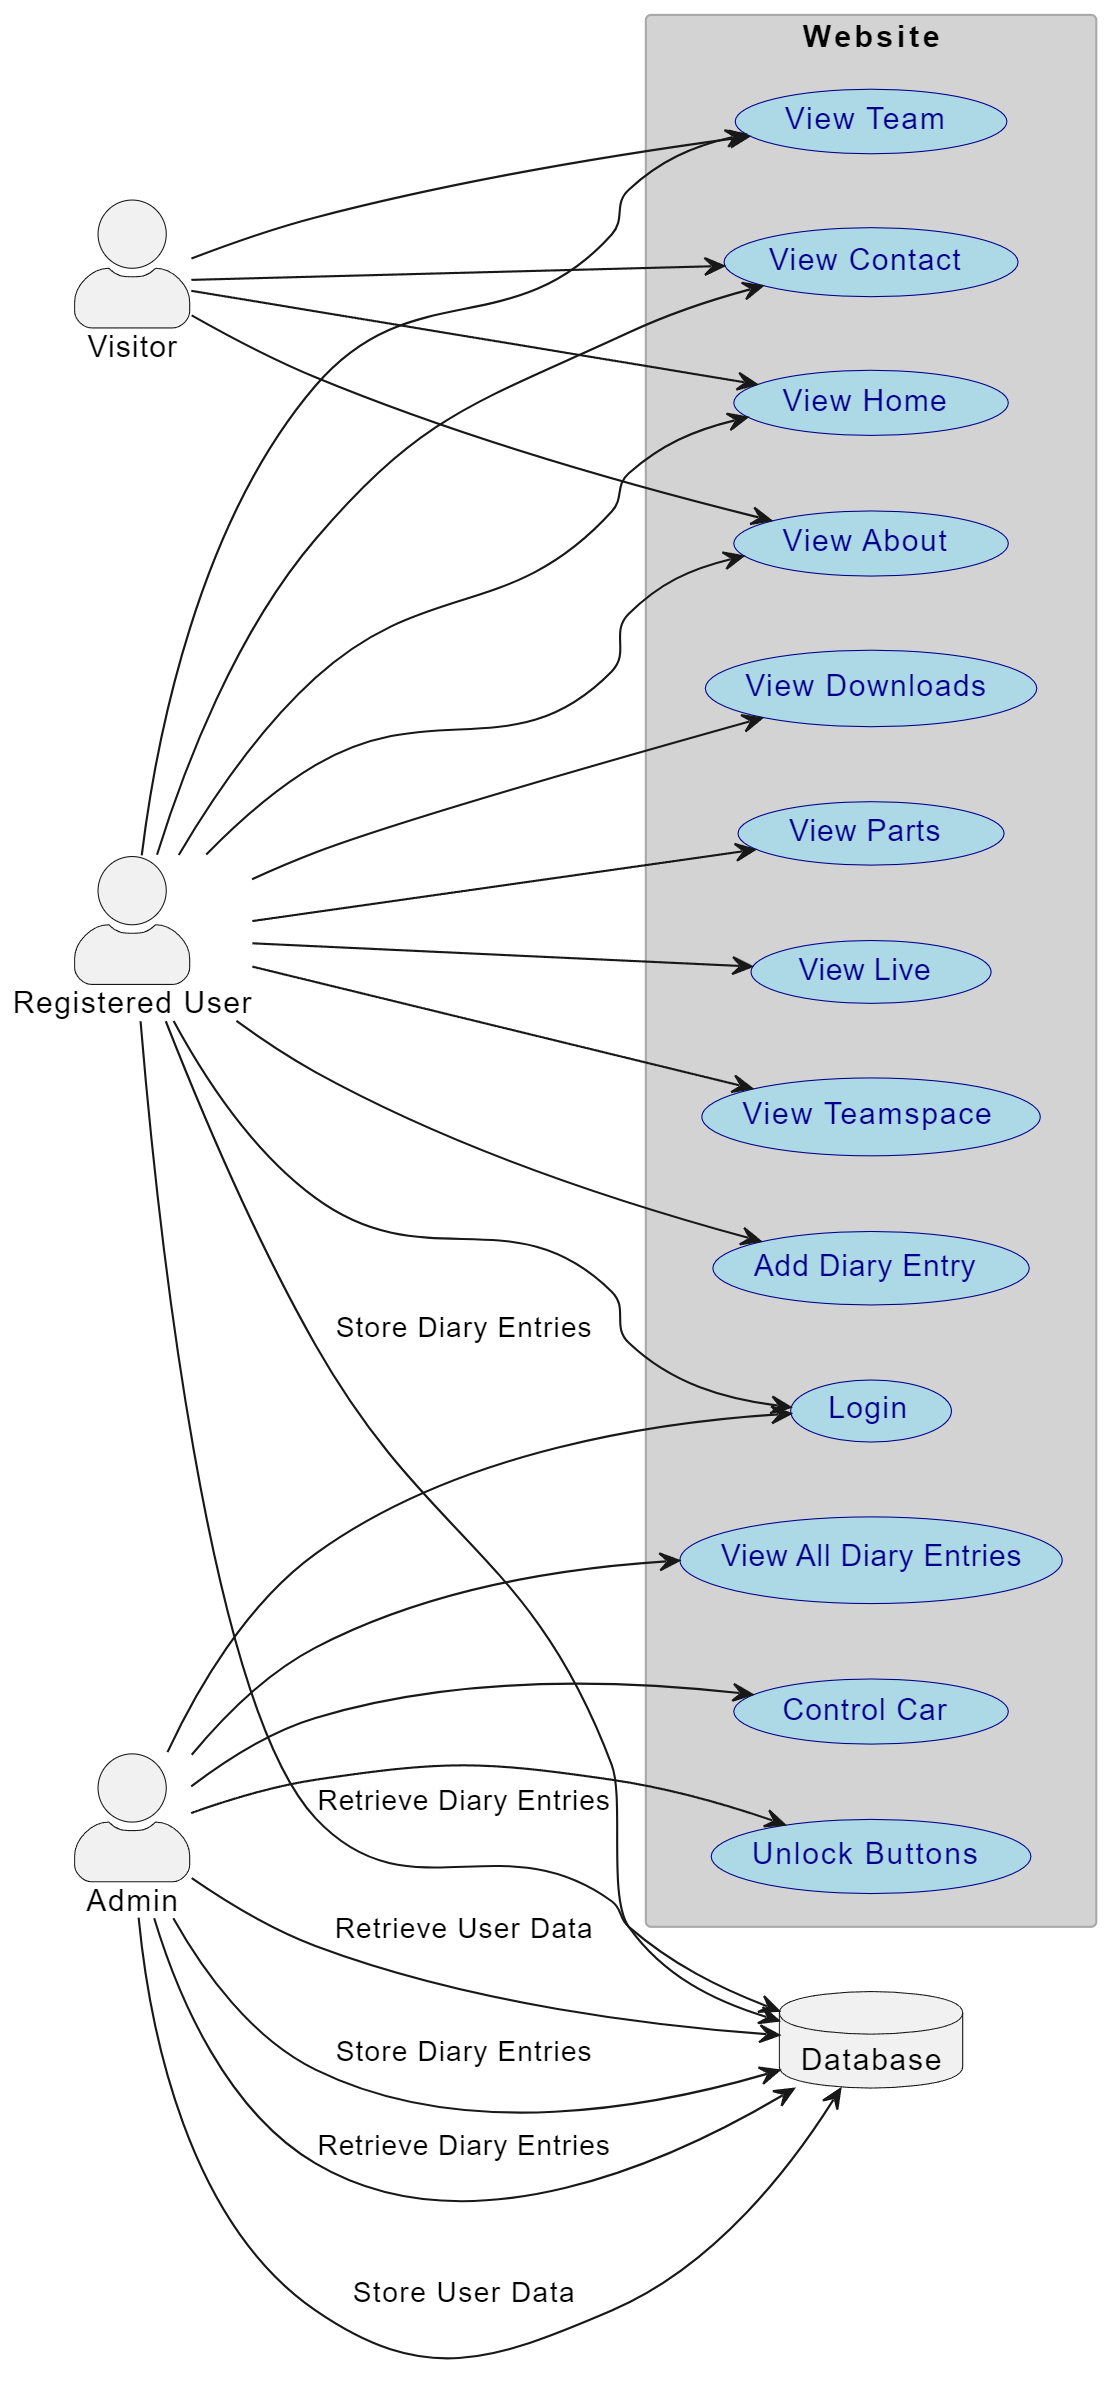
\includegraphics[width=0.52\textwidth]{Resources/diagram.png}
\caption{Usecase-Diagramm der Website-Interaktionen}
\end{figure}

\newpage

\subsection{Designraster und visuelle Gestaltung}

Das Design unserer Website ist von einem minimalistischen Ansatz geprägt, der sich auf das Wesentliche konzentriert und gleichzeitig ein einladendes und intuitives Benutzererlebnis bietet.

\subsubsection{Minimalistische Struktur}
Das Herzstück des Webdesigns ist die zentral positionierte, vertikale Menüleiste, die beim ersten Besuch der Website die alleinige Aufmerksamkeit auf sich zieht. Sie ist so konzipiert, dass sie das Bildschirmverhältnis im geschlossenen Zustand in drei gleich große Teile teilt, was eine harmonische Balance auf der Startseite schafft. Ein Klick auf eines der Menüelemente verlagert die Leiste nach links und öffnet den Inhalt des ausgewählten Menüpunkts auf der rechten Seite, im Verhältnis von etwa einem Drittel zu zwei Dritteln der Bildschirmbreite. Diese dynamische Bewegung verleiht der Seite eine lebendige Interaktivität und hält das Layout klar und fokussiert.

\subsubsection{Farbschema}
Die Hauptfarbe unserer Website ist ein sanftes Beige, repräsentiert durch das Farbquadrat nebenstehend, welches Ruhe und Wärme ausstrahlt und den minimalistischen Charakter unserer Website unterstreicht. Für einen starken Kontrast, der die Lesbarkeit insbesondere für Sehbehinderte erhöht, verwenden wir zusätzlich Schwarz in Texten und kritischen Interaktionselementen.

\noindent\raisebox{-0.7\height}{
\includegraphics[width=1cm]{Resources/color_sample.png}} \quad \raisebox{-0.7\height}{
\includegraphics[width=1cm]{Resources/color_sample_black.png}}

\subsubsection{Typografie und Lesbarkeit}
Die Typografie folgt dem Minimalismus der Seite, wobei klare, gut lesbare Schriftarten verwendet werden, die sowohl auf Bildschirmen als auch im Druck gut funktionieren. Große Schriftgrade und ausreichender Zeilenabstand gewährleisten eine hervorragende Lesbarkeit und Zugänglichkeit.

Als Hauptstandardschrift für Überschriften wurde \texttt{font-family: 'Cairo', sans-serif;} gewählt. Die Schriftart \textit{Cairo} ist bekannt für ihre moderne und klare Linienführung, die hilft, einen visuellen Eindruck von Ordnung und Sauberkeit zu vermitteln. Dies unterstützt den minimalistischen Ansatz der Website und fördert gleichzeitig eine starke visuelle Hierarchie, die es den Nutzern erleichtert, Inhalte schnell zu erfassen.

Ergänzend dazu wird \texttt{font-family: Arial, sans-serif;} für den Fließtext verwendet. \textit{Arial} ist eine extrem verbreitete und gut lesbare Schriftart, die aufgrund ihrer ausgezeichneten Lesbarkeit und ihrer unauffälligen Erscheinung auf einer Vielzahl von Geräten gut funktioniert. Dies trägt zur Konsistenz und Zugänglichkeit der Website bei, indem sichergestellt wird, dass Texte unter verschiedenen Betrachtungsbedingungen gut lesbar bleiben.

\subsubsection{Interaktionsdesign}
Das Interaktionsdesign ist so gestaltet, dass es sich nahtlos in die minimalistische Gestaltung einfügt. Die Übergänge sind glatt und die Benutzereingaben führen zu einer unmittelbaren und visuell ansprechenden Rückmeldung, was die Benutzererfahrung verbessert und ein Gefühl von Direktheit und Reaktionsfähigkeit vermittelt.

\subsubsection{Visuelle Hilfsmittel und Grafiken}
Die Verwendung von visuellen Hilfsmitteln und Grafiken ist sorgfältig dosiert. Sie ergänzen den Text, wo nötig, ohne die Benutzer von der Hauptbotschaft abzulenken. Die Grafiken sind so gestaltet, dass sie die Farbgebung aufgreifen und den Fokus auf die Interaktion verstärken.

\begin{figure}[h]
    \centering
    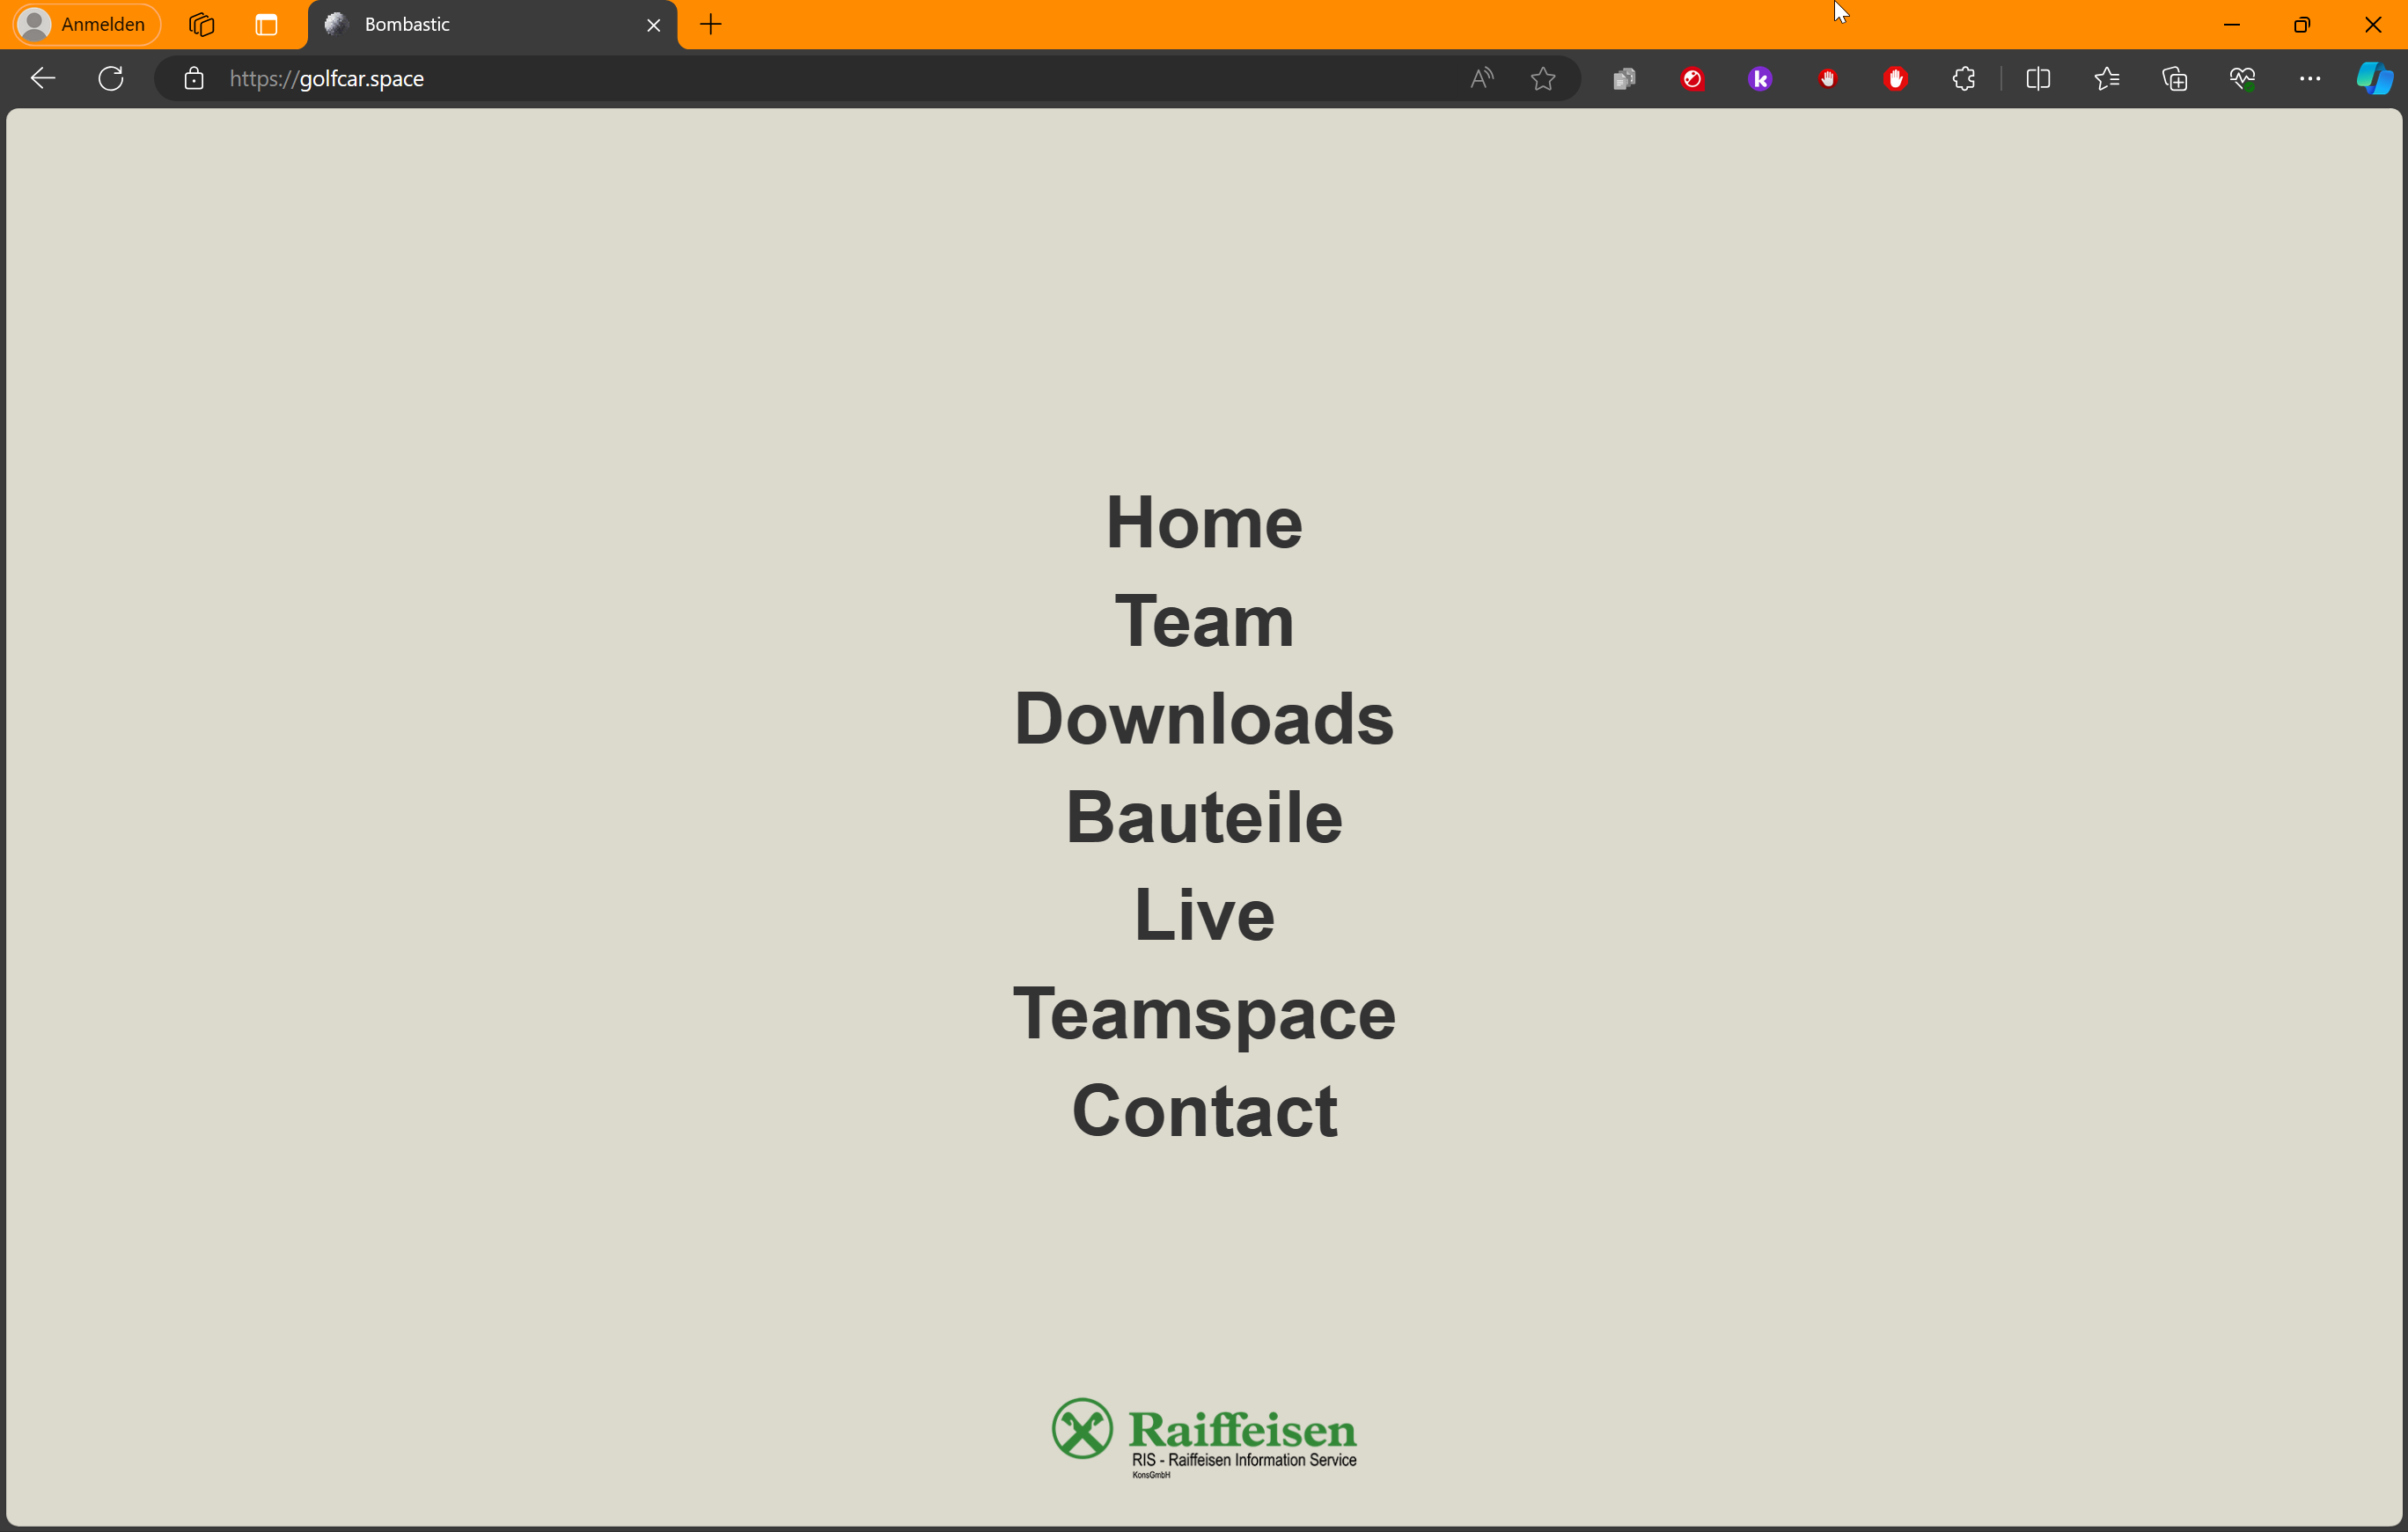
\includegraphics[width=\linewidth]{Resources/menu_screenshot.png}
    \caption{Screenshot des minimalistischen Menüs mit der Hauptfarbe im Hintergrund.}
    \end{figure}

%TODO: improve    
\subsection{Wirkung und Zielsetzung}

Die Gestaltung unserer Website zielt darauf ab, sowohl Benutzerfreundlichkeit als auch eine innovative Atmosphäre zu vermitteln. Unsere Vision ist es, eine futuristische Ästhetik zu schaffen, die sich in einer klaren, intuitiven Nutzerführung und einer sanften, ansprechenden Farbgestaltung widerspiegelt.

\subsubsection{Gesamteindruck und Emotionale Verbindung}
Beim Betreten der Website soll der Benutzer in eine Welt eintreten, die durch ein futuristisches Design geprägt ist, ohne dabei überladen zu wirken. Die zentrale Menüführung, unterstützt durch die weiche Farbgebung unseres Designs, lädt zum Entdecken und Verweilen ein, wobei die intuitive Benutzerführung das Engagement und die Interaktion fördert.

\subsubsection{Visionäre Kommunikation}
Die Vision des selbstfahrenden Golfcars wird durch minimalistische, aber ausdrucksstarke Grafiken kommuniziert, die die technologische Eleganz und die smarten Fähigkeiten des Autos hervorheben. Wir nutzen visuelle Metaphern, um die Innovation unseres Projekts zu betonen und die Stärken des Golfcars zu illustrieren.

\subsubsection{Call-to-Action}
Unser minimalistisches Menü fungiert als klarer Wegweiser für die Nutzeraktionen. Durch die einfache Auswahl der Menüpunkte wird der Benutzer ermutigt, die verschiedenen Aspekte unseres Projekts zu erkunden, von den technischen Details bis hin zur Live-Steuerung des Golfcars.

\subsubsection{Visuelles Konzept}
Für die bildliche Darstellung könnten wir abstrakte, technologieinspirierte Linienmuster verwenden, die Bewegung und Vernetzung symbolisieren. Grafiken von stilisierten Netzwerkdiagrammen oder schematischen Darstellungen des Golfcars könnten die futuristische und innovative Seite unseres Projekts betonen. Diese visuellen Elemente würden die Prinzipien des minimalistischen Designs aufgreifen und gleichzeitig die fortschrittliche Technik des selbstfahrenden Golfcars visualisieren.

%\begin{figure}[h]
%\centering
%\includegraphics[width=0.5\textwidth]{tech_graphic.png}
%\caption{Stilisierte Darstellung der Vernetzung und Technologie des Golfcars.}
%\end{figure}


\subsection{Ergonomie und Benutzerfreundlichkeit}

Die Ergonomie und Benutzerfreundlichkeit unserer Website sind zentrale Aspekte des Designs und der Entwicklung. Ziel ist es, allen Nutzern eine intuitive und angenehme Erfahrung zu bieten.

\subsubsection{Interaktionsdesign und Navigation}
Die Navigation auf unserer Website ist intuitiv gestaltet, um sicherzustellen, dass Benutzer schnell und effizient die gewünschten Informationen finden. Interaktive Elemente wie Buttons und Links sind klar erkennbar: Buttons sind deutlich als solche gestaltet, und Links sind traditionell blau und unterstrichen, um ihre Funktion offensichtlich zu machen. Hover-Effekte auf bestimmten Elementen bieten zusätzliche Informationen, was die Usability erhöht und Benutzern hilft, die Funktionalitäten besser zu verstehen.

\subsubsection{Feedback-Mechanismen}
Um eine interaktive und responsive Nutzererfahrung zu gewährleisten, implementiert die Website effektive Feedback-Mechanismen. Bei fehlerhaften Anmeldeversuchen, wie zum Beispiel durch die Eingabe eines falschen Benutzernamens oder Passworts, gibt der Browser sofort eine klare Fehlermeldung aus. Diese sofortige Rückmeldung hilft Benutzern, Korrekturen vorzunehmen und verbessert die allgemeine Benutzerinteraktion.

\subsubsection{Unterstützung für Sehbehinderte}
Auch die Bedürfnisse sehbehinderter Nutzer werden berücksichtigt. Überschriften und Zwischenüberschriften sind groß und gut lesbar gestaltet, mit hohem Kontrast, um die Lesbarkeit zu maximieren. Diese Designentscheidungen tragen dazu bei, die Zugänglichkeit unserer Website zu erhöhen.

\subsubsection{Optimierung der Ladezeiten}
Obwohl spezifische Maßnahmen zur Optimierung der Ladezeiten noch in Entwicklung sind, ist die Website bereits so konzipiert, dass sie effizient und schnell lädt. Zukünftige Updates werden weitere Verbesserungen in diesem Bereich bringen, um eine nahtlose Benutzererfahrung zu gewährleisten.

\subsubsection{Zukünftige Verbesserungen}
Wir planen, die Ergonomie und Benutzerfreundlichkeit kontinuierlich zu verbessern, indem wir Benutzerfeedback sammeln und analysieren. Die Umsetzung von Benutzervorschlägen wird uns helfen, die Website weiter zu optimieren und eine noch bessere Benutzererfahrung zu bieten.

\subsection{Grundlegende Überlegungen bei der Projektierung}

Bei der Entwicklung und dem Betrieb unserer Website für das selbstfahrende Miniatur-Golfcar-Projekt sind verschiedene Schlüsselfaktoren zu berücksichtigen, die für den Erfolg und die Reichweite unserer Online-Präsenz entscheidend sind.

\subsubsection{Werbung und Sichtbarkeit}

Um unser Projekt einem breiteren Publikum bekannt zu machen, planen wir den Einsatz von Google AdSense, gezielte Werbekampagnen auf Instagram sowie die Verteilung von Flyern in Schulen. Eine Kooperation mit Bildungseinrichtungen bietet sich an, um das Interesse von Lehrern und Schülern zu wecken und eine pädagogische Partnerschaft aufzubauen.

\subsubsection{Hosting und Zugänglichkeit}

In der Anfangsphase wird unsere Website auf einem Linux-Server unserer Schule gehostet, was den Zugriff zunächst auf das schulinterne Netzwerk beschränkt. Diese Vorgehensweise bietet einen kontrollierten Rahmen für die ersten Tests und die Weiterentwicklung der Website. In der Zukunft ist geplant, die Website auf einer öffentlichen Domain zu hosten, um das Projekt für alle Interessierten zugänglich zu machen.

\subsubsection{Qualitätssicherung und Versionierung}

Die Qualitätssicherung ist ein kontinuierlicher Prozess, der in Zusammenarbeit zwischen dem Projektleiter und den Webentwicklern durchgeführt wird. Wir nutzen Git für die Versionierung unserer Inhalte, um eine konsistente Weiterentwicklung und Fehlerbehebung zu gewährleisten. Im Impressum der Website wird die Aktualität der Inhalte durch Angabe des letzten Aktualisierungsdatums kommuniziert.

\subsubsection{Aktualisierung der Inhalte}

Neue Erkenntnisse, Fortschritte im Projekt und relevante Neuigkeiten werden regelmäßig auf der Website veröffentlicht, um unsere Besucher auf dem Laufenden zu halten. Diese Transparenz fördert das Vertrauen und die Einbindung der Community.

\subsubsection{Suchmaschinenoptimierung (SEO)}

Um die Auffindbarkeit unserer Website zu verbessern, setzen wir auf die Integration von Meta-Tags, die relevante Schlüsselwörter enthalten. Zusätzlich nutzen wir Google Analytics, um die Effektivität unserer Online-Präsenz zu bewerten und zu optimieren.

\paragraph{Meta-Tags und ihre Bedeutung}
Meta-Tags spielen eine entscheidende Rolle bei der Suchmaschinenoptimierung. Sie helfen Suchmaschinen, den Inhalt der Seiten besser zu verstehen und korrekt zu indizieren. Hier ein Beispiel der auf unserer Website verwendeten Meta-Tags:

\begin{lstlisting}
    <meta charset="UTF-8">
    <meta name="description" content="Schulprojekt Golfcar der Gruppe 6B-Engineering. Das Ziel: Ein selbstfahrendes Auto zu bauen, das einen Golfball automatisch in eine Box befoerdert">
    <meta name="keywords" content="Golfcar, Autonomous Car, ... , Educational Robotics, Open Source Hardware, IoT, Internet of Things, Maker Movement, Tech DIY, Electronic Components, Coding, Software Development, Hardware Programming">
    <meta name="robots" content="index, follow">
    <meta name="viewport" content="width=device-width, initial-scale=1.0">
    <meta name="author" content="6B Engineering">
    <!-- Open Graph Tags -->
    <meta property="og:title" content="6B-Engineering">
    <meta property="og:description" content="Schulprojekt Golfcar der Gruppe 6B-Engineering. Das Ziel: Ein selbstfahrendes Auto zu bauen, das einen Golfball automatisch in eine Box befoerdert">
\end{lstlisting}

\paragraph{Nutzung von Google Analytics}
Google Analytics hilft uns, die Besucherströme zu analysieren und die Wirkung unserer SEO-Maßnahmen zu verstehen. Diese Daten sind entscheidend für die kontinuierliche Optimierung unserer Inhalte und die Steigerung der Benutzerfreundlichkeit unserer Website.

\begin{figure}[h]
    \centering
    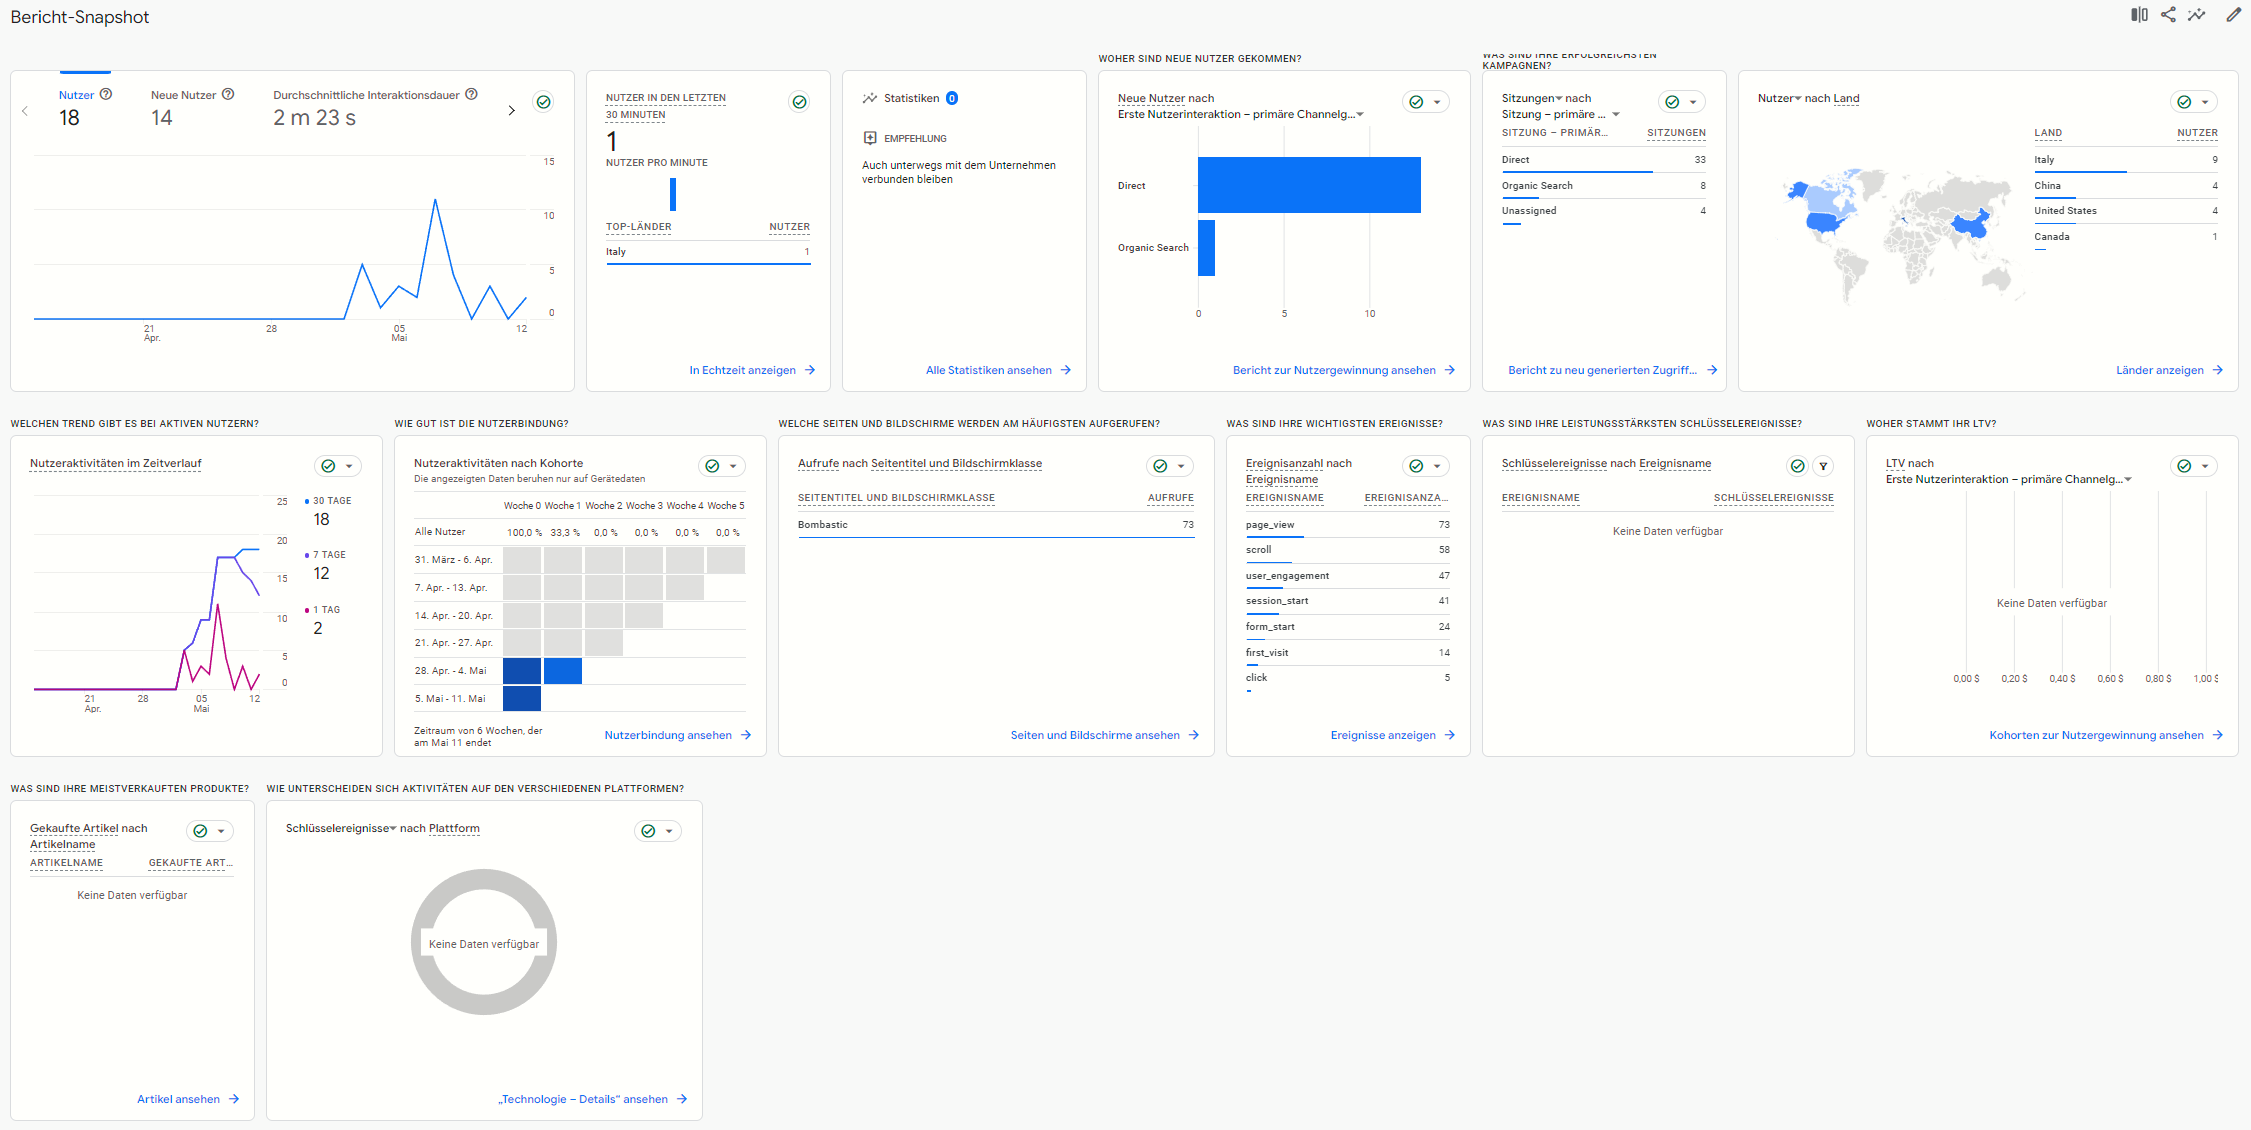
\includegraphics[width=\textwidth]{Resources/SEO_snapshot.png}
    \caption{Google Analytics Snapshot: Überblick über Nutzerinteraktionen und Engagement.}
\end{figure}

\newpage

\paragraph{Weitere Analyseergebnisse}
Die weiteren SEO-Analysebilder geben Einblick in verschiedene Nutzungsaspekte unserer Website:

\begin{figure}[h]
    \centering
    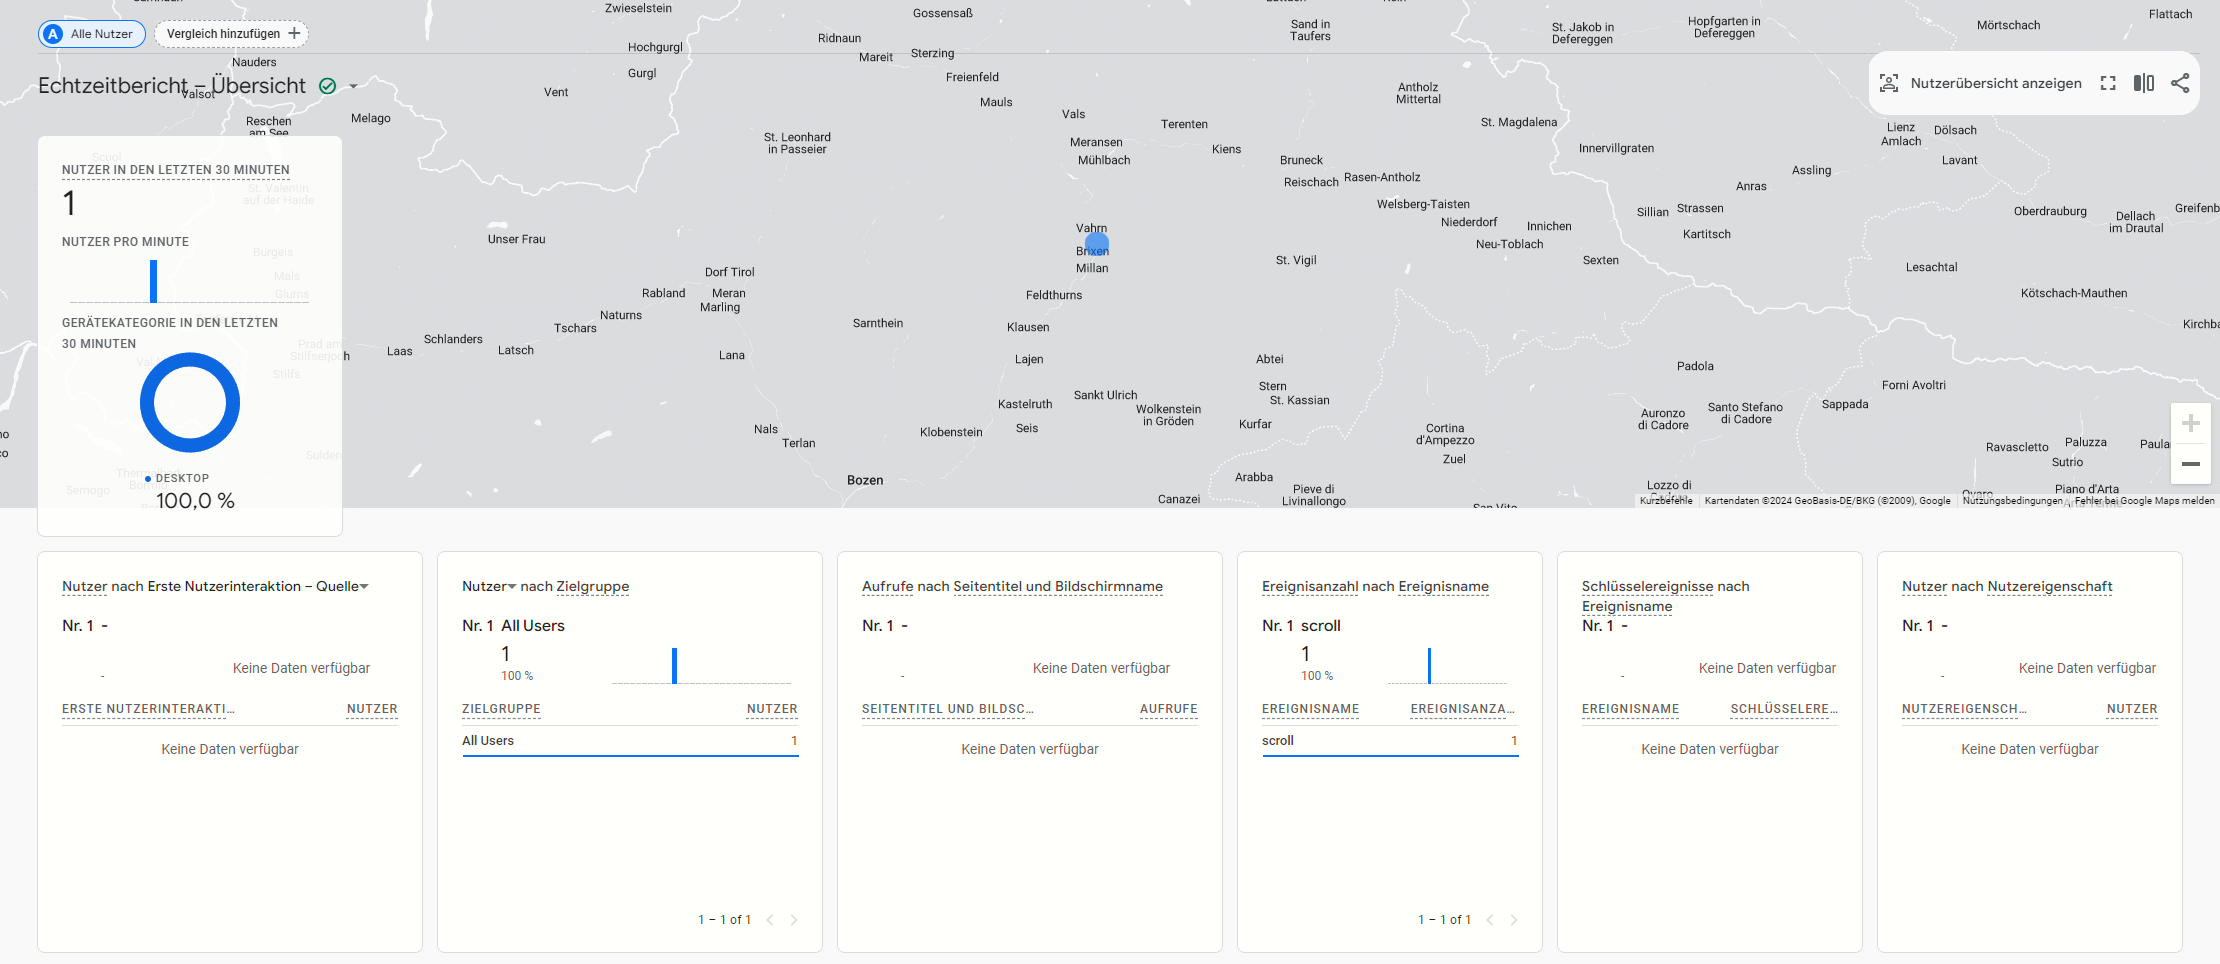
\includegraphics[width=\textwidth]{Resources/SEO_echtzeit.png}
    \caption{Echtzeit-Analyse: Aktive Nutzer und geographische Verteilung.}
\end{figure}

\begin{figure}[h]
    \centering
    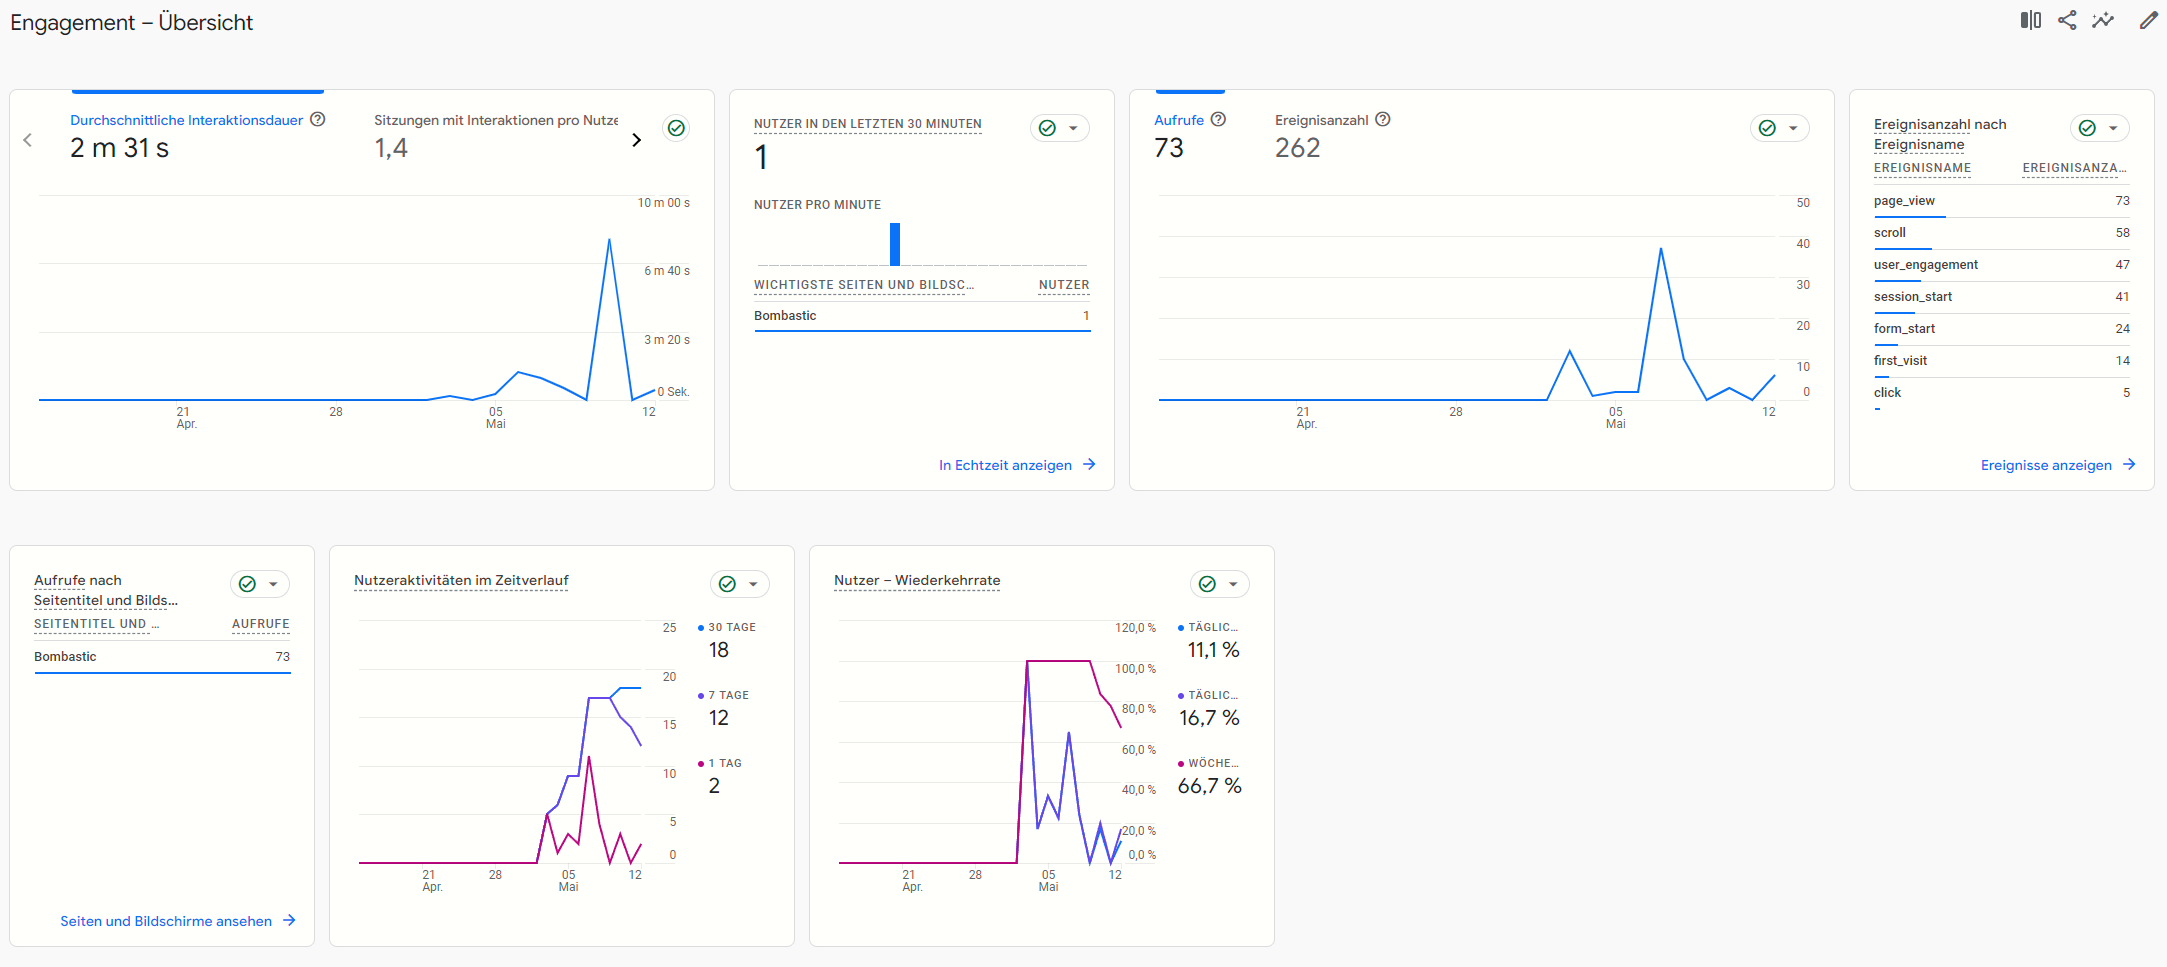
\includegraphics[width=\textwidth]{Resources/SEO_engagement.png}
    \caption{Nutzerengagement und Interaktionstiefe.}
\end{figure}

\newpage

\begin{figure}[h]
    \centering
    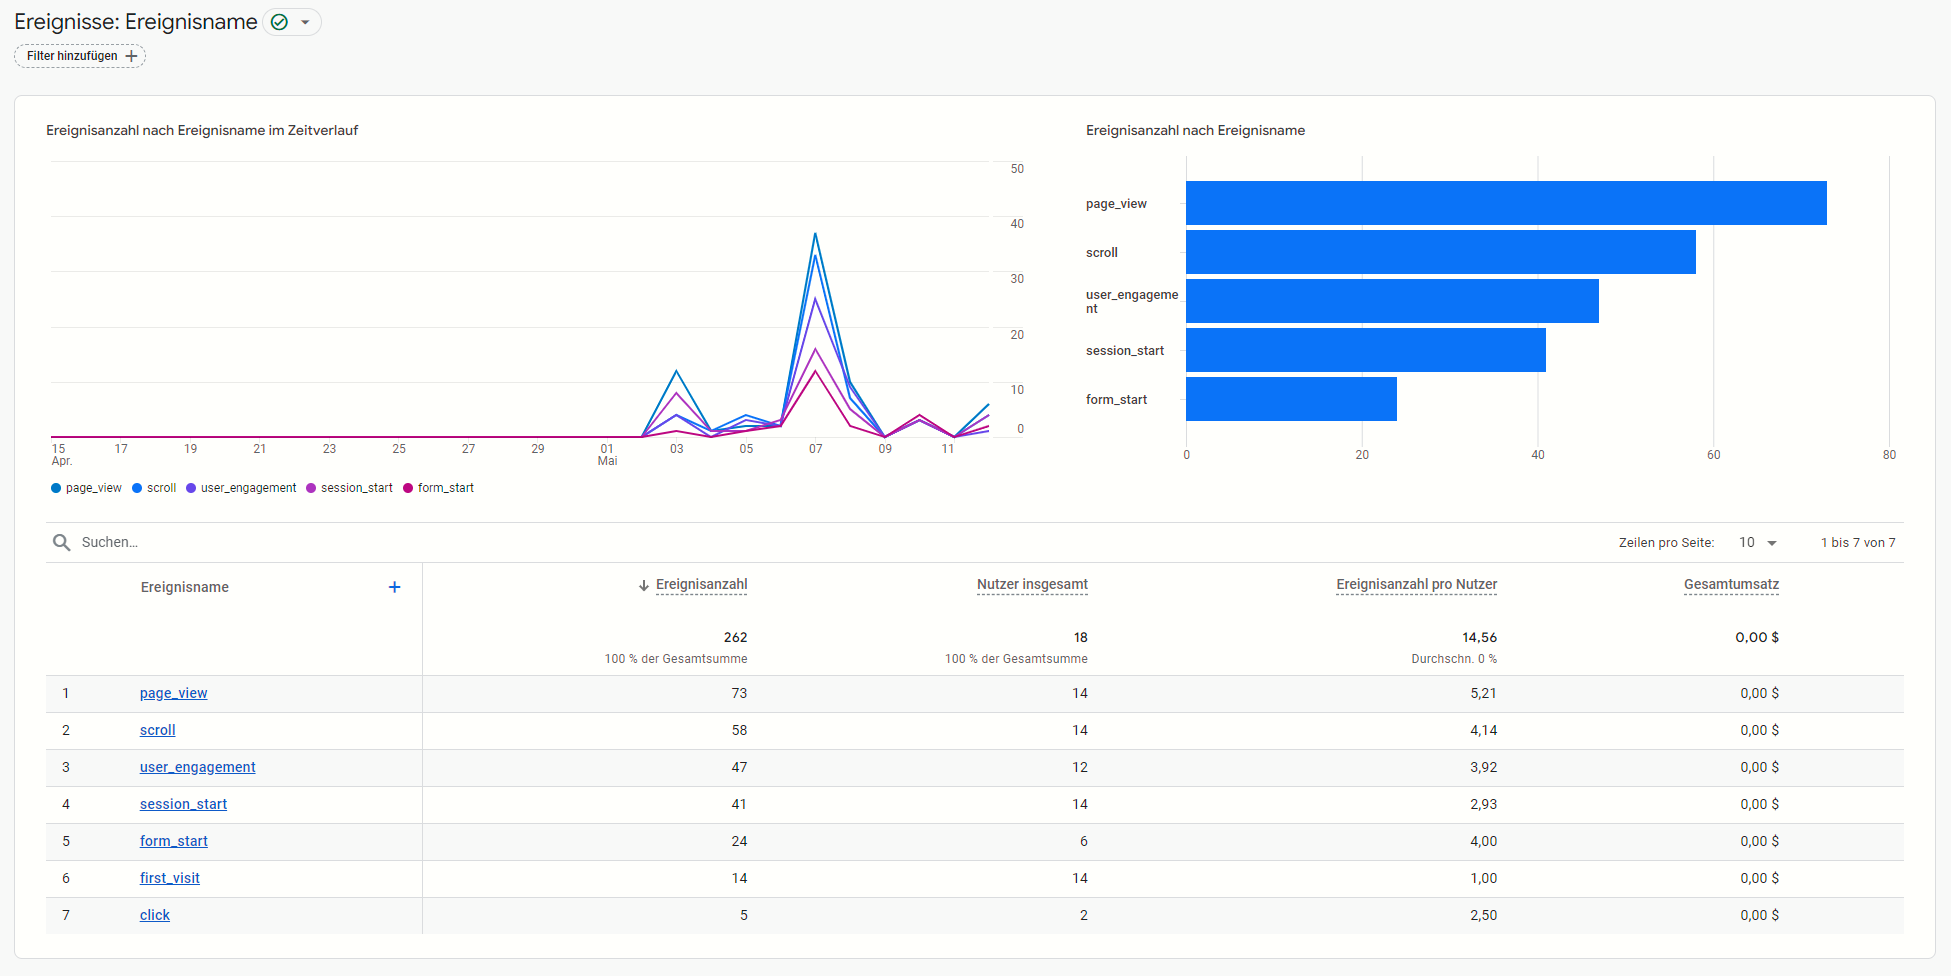
\includegraphics[width=\textwidth]{Resources/SEO_ergebnisse.png}
    \caption{Analyse der Ergebnisse und Nutzerfeedback.}
\end{figure}

\begin{figure}[h]
    \centering
    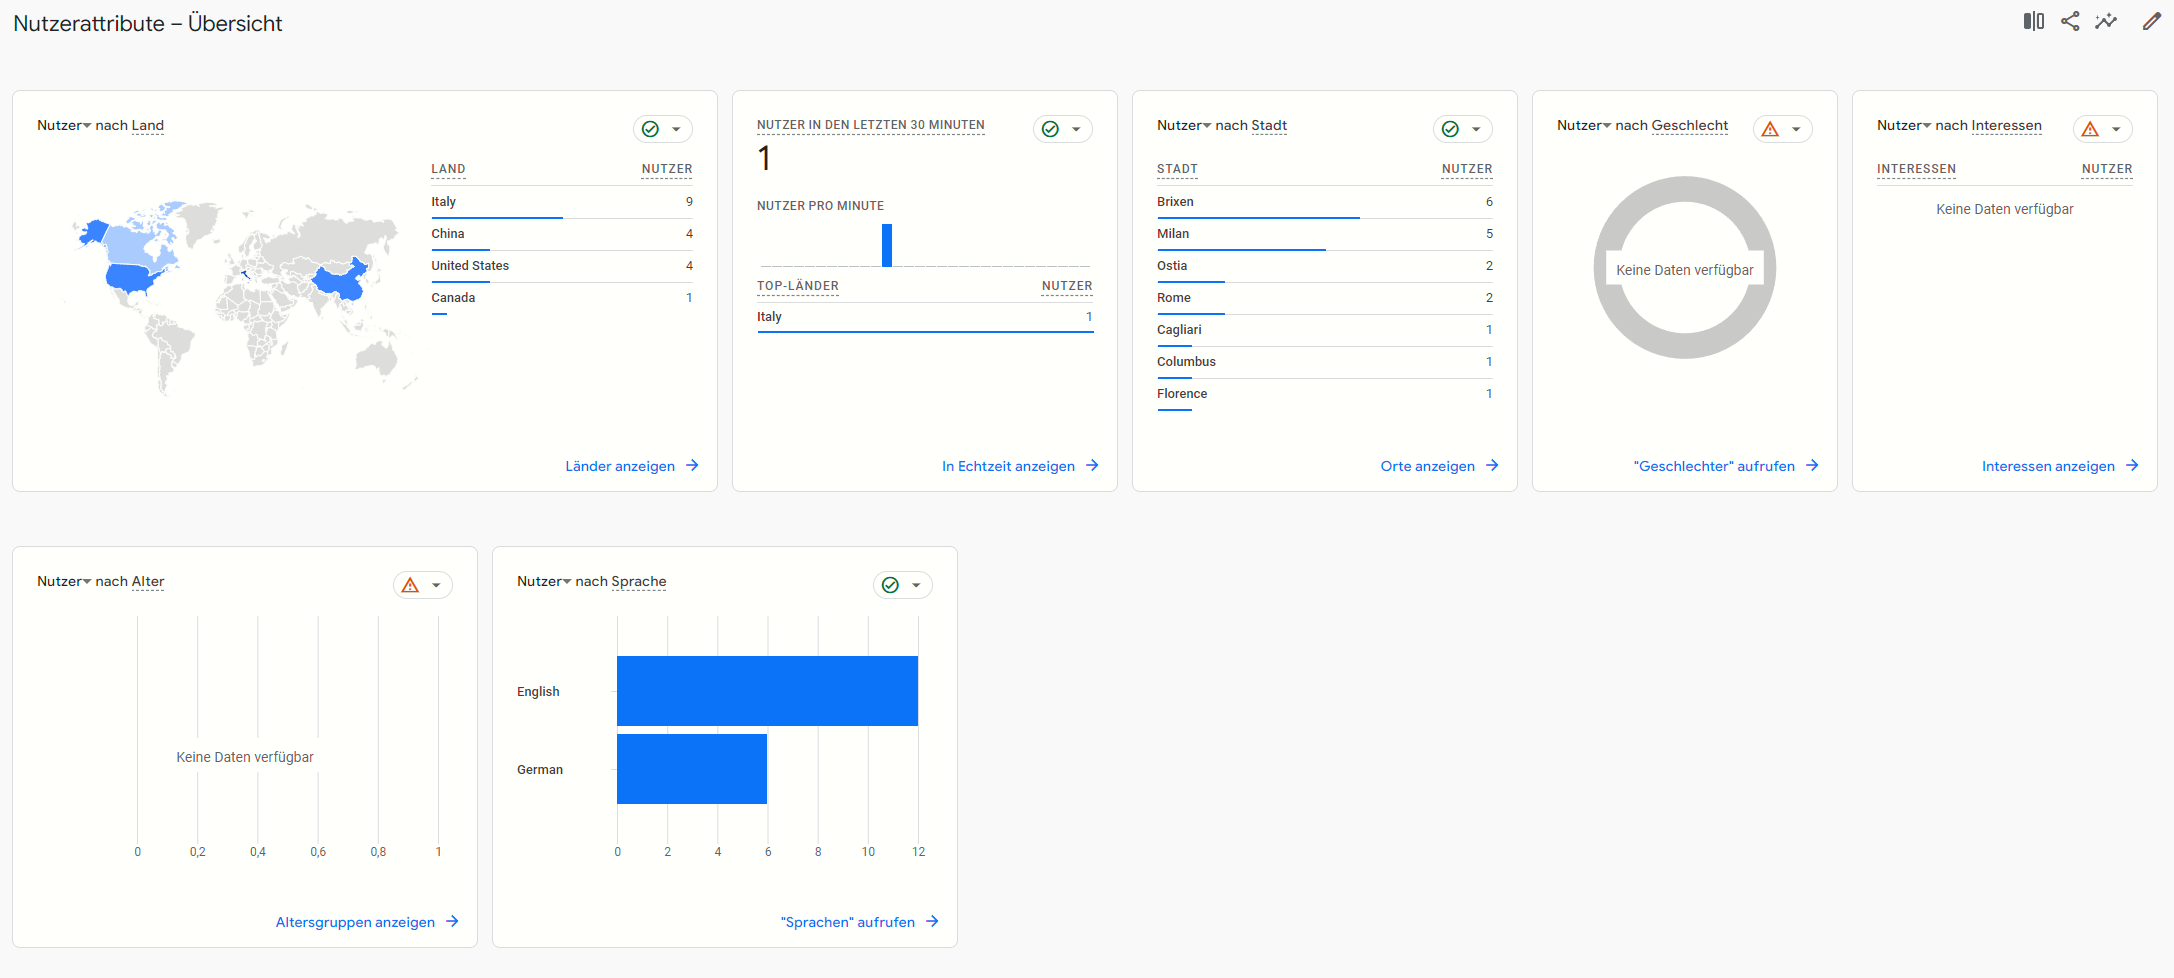
\includegraphics[width=\textwidth]{Resources/SEO_nutzerattribute.png}
    \caption{Detaillierte Attribute der Nutzer.}
\end{figure}

\newpage

\begin{figure}[h]
    \centering
    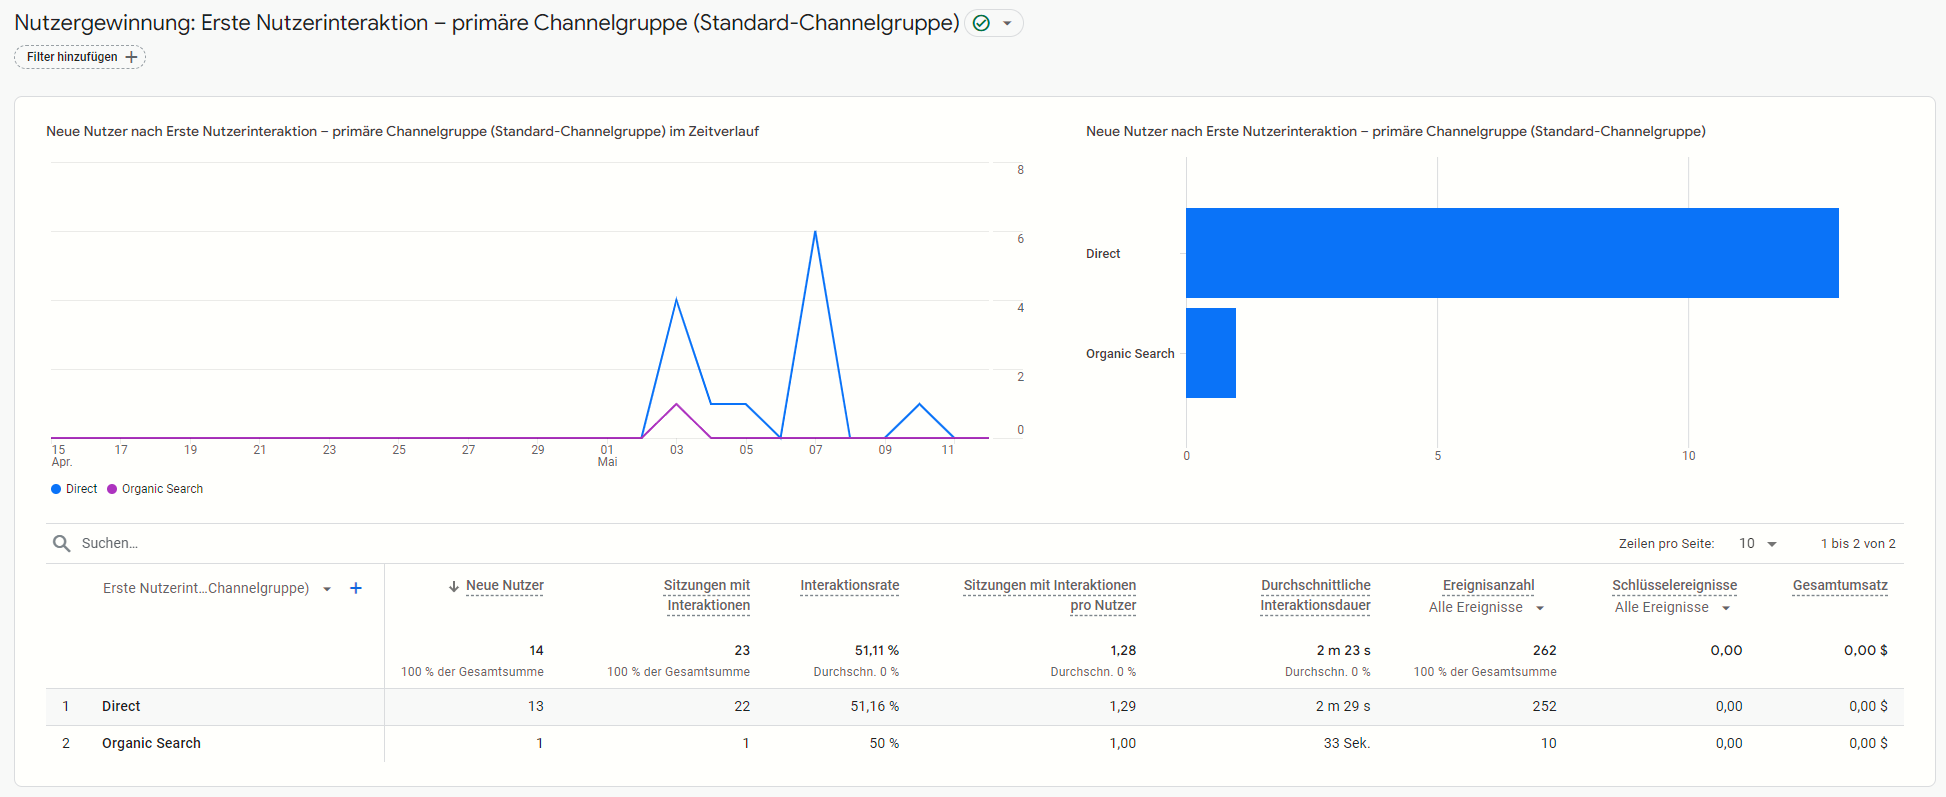
\includegraphics[width=\textwidth]{Resources/SEO_nutzergewinnung.png}
    \caption{Methoden der Nutzergewinnung und deren Effektivität.}
\end{figure}

\begin{figure}[h]
    \centering
    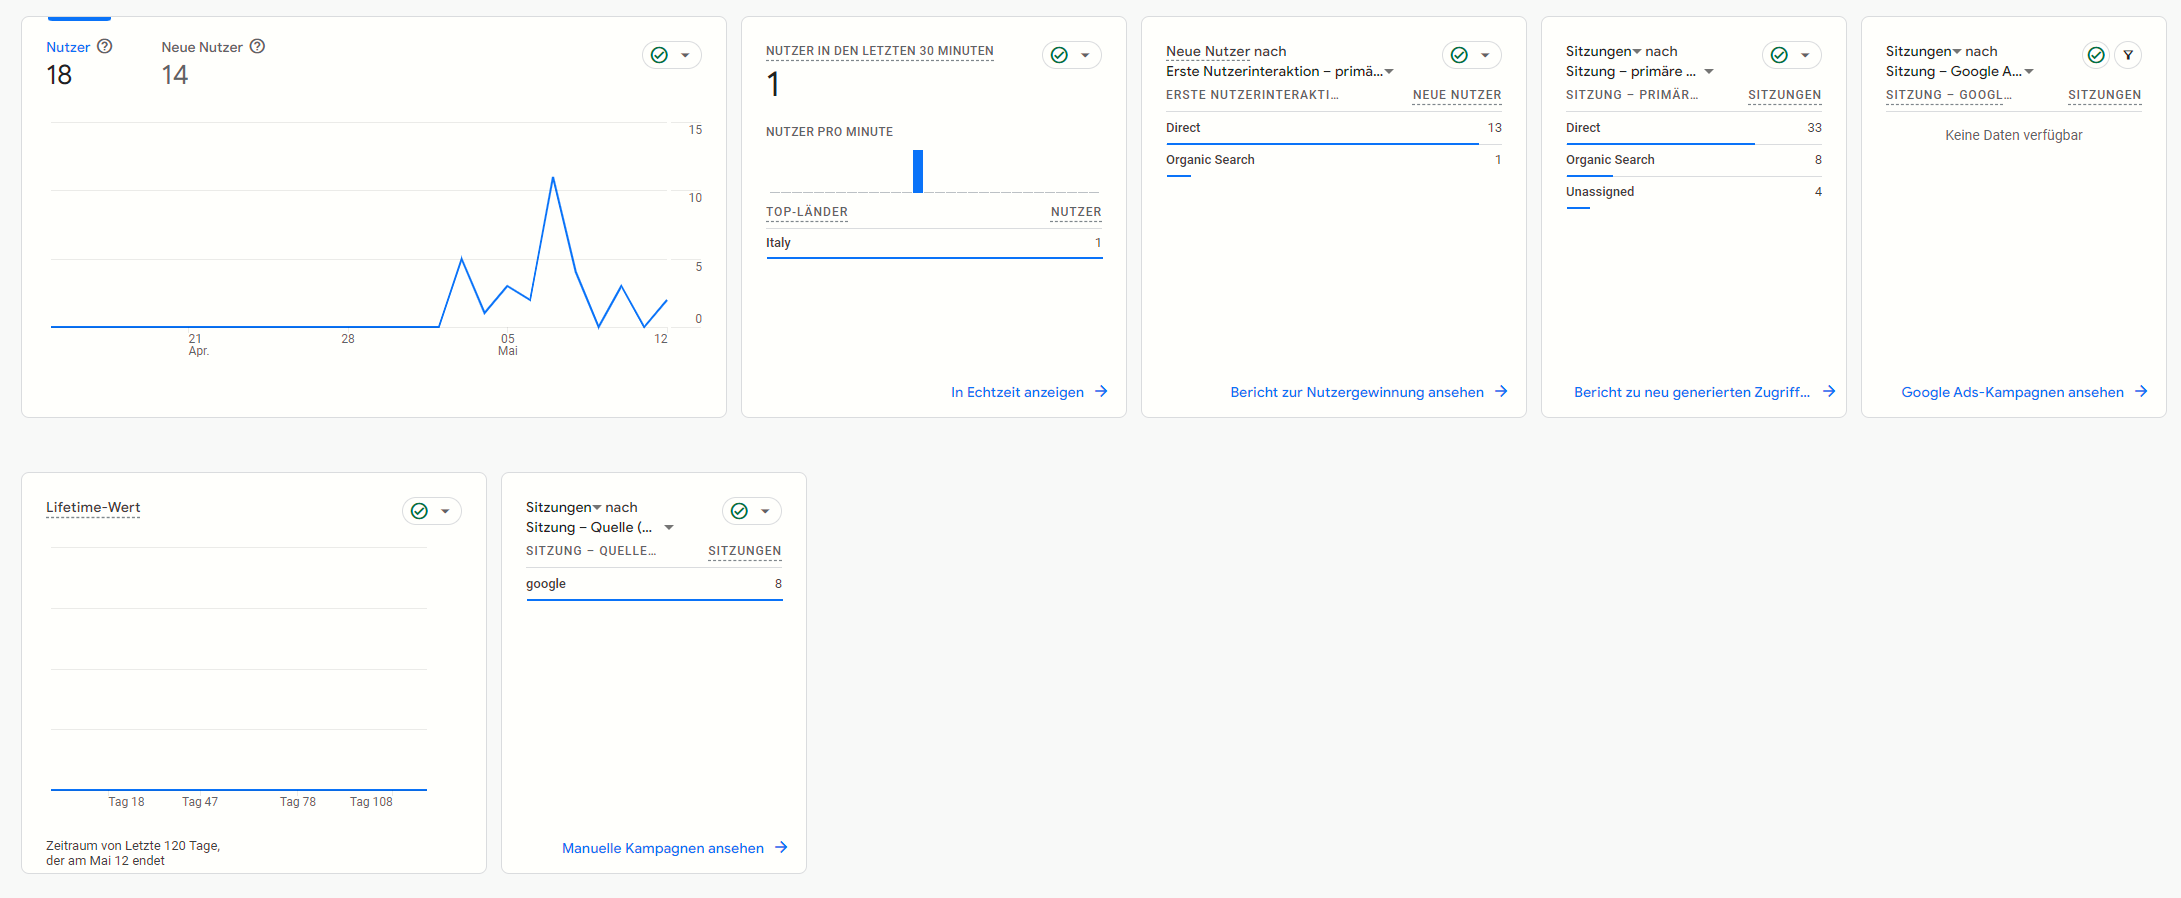
\includegraphics[width=\textwidth]{Resources/SEO_uebersicht.png}
    \caption{Umfassende Übersicht der SEO-Leistung und Nutzerdaten.}
\end{figure}

Diese umfangreichen Daten erlauben uns, fundierte Entscheidungen über zukünftige Anpassungen und Verbesserungen zu treffen, um die Besuchererfahrung weiter zu optimieren und unsere Website effektiv zu präsentieren.

\newpage

\subsection{Abschluss und Ausblick}

\subsubsection{Zusammenfassung der Ziele}
Die primären Ziele unserer Website waren die Präsentation des Teams, die Darstellung der Vision unseres selbstfahrenden Golfcar-Projekts sowie die Bereitstellung einer interaktiven Steuerung des Fahrzeugs über die Website. Diese Ziele wurden erfolgreich umgesetzt, was die Funktionalität und den innovativen Charakter unserer Plattform unterstreicht.

\subsubsection{Herausforderungen und Lösungen}
Während der Entwicklungsphase traten mehrere technische und organisatorische Herausforderungen auf:
\begin{itemize}
    \item \textbf{JSON-Dateien:} Anfängliche Schwierigkeiten im Umgang mit JSON-Dateien führten zu fehlerhaften Einträgen. Durch Implementierung zusätzlicher Kontrollabfragen und Formatierungschecks konnten diese Probleme behoben werden.
    \item \textbf{Edit Button:} Fehler durch die Verwendung von Anführungszeichen in Tagebucheinträgen wurden durch verbesserte Datenvalidierung gelöst.
    \item \textbf{Sicherheitsvorfall:} Nach einem Sicherheitsvorfall, verursacht durch einen Brute-Force-Angriff, haben wir die Sicherheitsmaßnahmen verschärft, indem wir Ports geändert, Anmeldedaten aktualisiert und automatische Sperrmechanismen für wiederholte Fehlanmeldungen (basierend auf der Software \textit{fail2ban}) implementiert haben.
\end{itemize}

\subsubsection{Feedback und Evaluation}
Das Feedback von Freunden und Klassenkameraden war entscheidend für die Optimierung der Website. Ihre Rückmeldungen zur Benutzerfreundlichkeit halfen uns, die Navigation und die allgemeine Benutzererfahrung zu verbessern.

\subsubsection{Langfristige Vision und zukünftige Entwicklungen}
Die langfristige Vision des Projekts ist die Veröffentlichung des gesamten Quellcodes auf GitHub nach der Projektvorstellung. Dies wird die Offenheit und Zugänglichkeit unserer Entwicklungsarbeit fördern und Interessierten ermöglichen, an der Weiterentwicklung teilzunehmen oder aus unseren Erfahrungen zu lernen. Aktuell sind keine weiteren spezifischen Ziele oder Meilensteine geplant.

\subsection{Aufruf zum Handeln}
Wir laden die Community ein, uns weiteres Feedback zu geben und sich an der Diskussion und Weiterentwicklung unseres Projekts zu beteiligen. Ihre Einsichten sind wertvoll für die fortlaufende Verbesserung und Anpassung unserer Website.

\subsection{Anhang}


\subsection{Literaturverzeichnis}
Das Literaturverzeichnis enthält alle referenzierten Quellen.


\section{Hosting der Website}
\subsection{Server und Hosting-Details}
Unsere Website wird auf einem vServer (VPS) gehostet, der bei noez.de angemietet ist. Dies bietet uns eine kostengünstige, aber leistungsfähige Lösung für das Hosting mit umfangreichen Konfigurationsmöglichkeiten. Die Primär-IP unseres Servers lautet 5.231.1.40, und wir haben umfassenden Zugriff auf das Servermanagement über ein benutzerfreundliches Webinterface.

\subsubsection{Technische Spezifikationen}
Der Server wird von einem Linux Ubuntu System betrieben und verfügt über 1020.05 MB RAM und eine CPU-Auslastung, die selten 5\% überschreitet, was auf eine effiziente Nutzung der Ressourcen hinweist. Der Trafficverbrauch liegt bei 8.06 GB von einem verfügbaren Volumen von 1000 GB pro Monat, was darauf hindeutet, dass wir gut innerhalb unserer Kapazitätsgrenzen operieren.

\subsubsection{Skalierbarkeit und Zugriffsmanagement}
Einer der Hauptvorteile unseres VPS ist die problemlose Skalierbarkeit. Durch einfaches Upgraden auf einen besseren Plan können wir die Serverressourcen je nach Bedarf erhöhen. Der volle Zugriff auf den Server mit Root-Rechten ermöglicht es uns, jederzeit Anpassungen vorzunehmen oder zusätzliche Dienste zu integrieren. Die Verwaltung des Servers erfolgt durch einen dedizierten Account, der ausschließlich von einer dafür spezialisierten Person unseres Teams gehandhabt wird.

\subsubsection{Sicherheit und Monitoring}
Die Details zu den Sicherheitsvorkehrungen und dem Monitoring unseres Servers sind in Abschnitt 5.8.2 des Berichts ausführlich dargestellt. Dort werden die Maßnahmen beschrieben, die nach einem Sicherheitsvorfall ergriffen wurden, einschließlich der verstärkten Sicherheitsprotokolle und der Nutzung von Fail2Ban.

\subsubsection{SEO und Google Analytics}
Die Nutzung unseres Servers ermöglicht auch die effektive Implementierung von SEO-Strategien und die Integration von Google Analytics. Diese Tools sind essenziell, um die Sichtbarkeit unserer Website zu erhöhen und detaillierte Einblicke in das Verhalten der Besucher zu erhalten. Weitere Informationen hierzu finden sich in Abschnitt 5.7.5 des Berichts.

\begin{figure}[h]
\centering
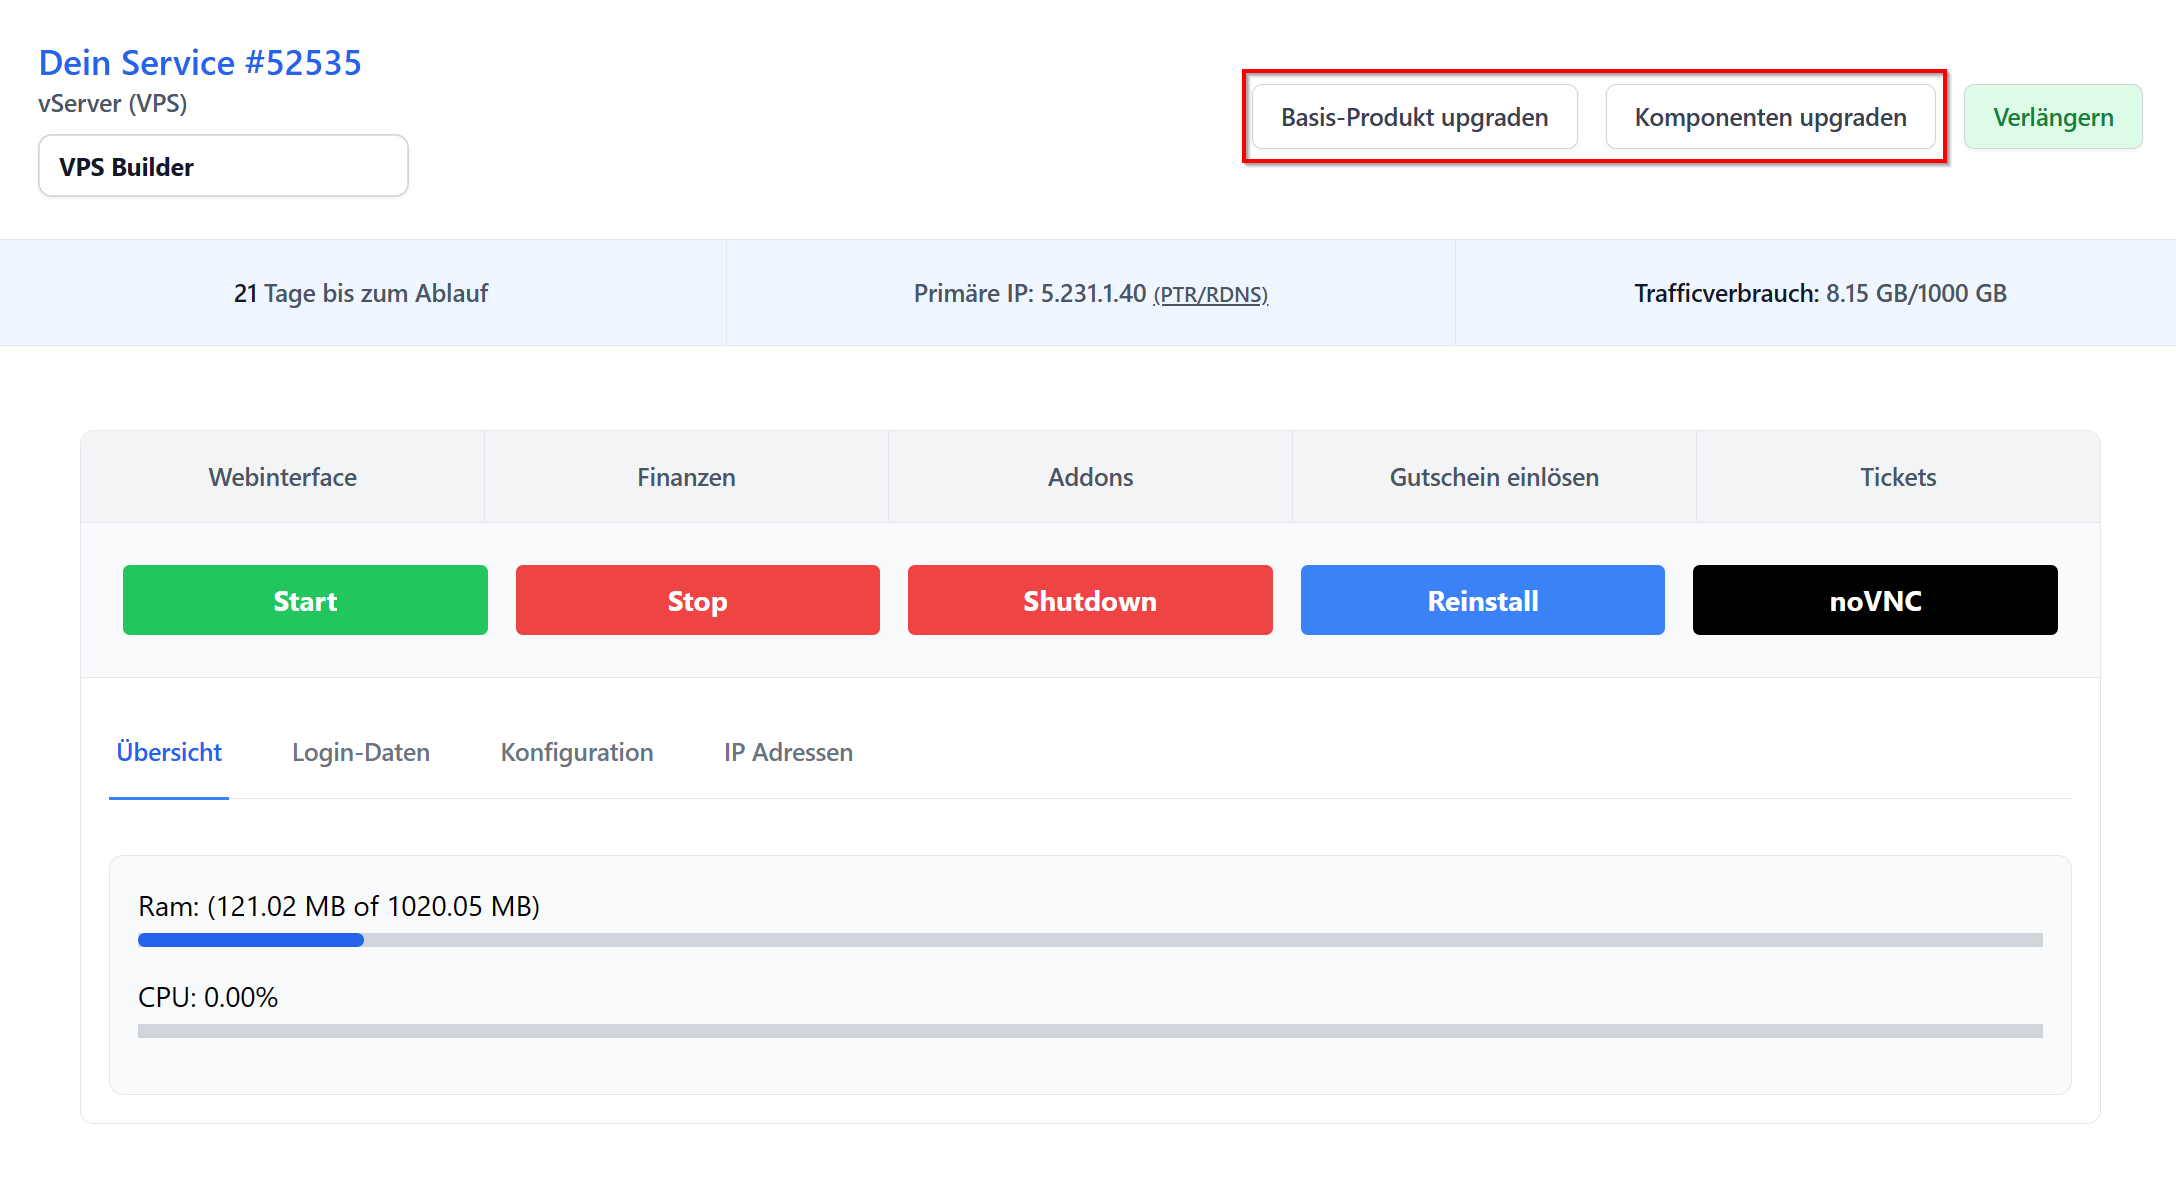
\includegraphics[width=1\textwidth]{Resources/hosting.png}
\caption{Screenshot des Server-Dashboards, der die Übersicht und Kontrolle des Hostings visualisiert.}
\end{figure}

Die robuste und flexible Hosting-Lösung stellt sicher, dass unsere Website nicht nur zuverlässig läuft, sondern auch gut auf zukünftiges Wachstum und zusätzliche Anforderungen vorbereitet ist.


\section{Abschlussbericht}
\subsection{Zusammenfassung der Projektziele}
Das Projektziel war die Entwicklung eines selbstfahrenden Miniatur-Golfcars, das in der Lage ist, Golfbälle autonom zu erkennen, aufzunehmen und an einem definierten Ort abzulegen. Die Website diente als Plattform zur Präsentation des Projekts, zur Bereitstellung von Informationen und zur Interaktion mit dem Fahrzeug über eine Live-Steuerung.

\subsection{Erfolge und Herausforderungen}
\subsubsection{Technische Herausforderungen und Lösungen}
Die Konstruktion des Fahrzeugs und die Entwicklung der Website brachten verschiedene technische Herausforderungen mit sich:
\begin{itemize}
    \item \textbf{Platzierung der Ultraschallsensoren:} Die optimale Platzierung der Sensoren erwies sich als schwierig, wurde jedoch durch wiederholte Tests und Anpassungen des Chassis erfolgreich gelöst.
    \item \textbf{Verwendung von Autodesk Inventor:} Trotz der Komplexität des Programms ermöglichte die Verwendung von professioneller CAD-Software eine präzise und modulare Konstruktion, die entscheidend für den Erfolg des Projekts war.
    \item \textbf{Sicherheitsvorfall:} Ein Brute-Force-Angriff führte zu einer Überarbeitung der Sicherheitsmaßnahmen. Durch die Implementierung von Fail2Ban und die Aktualisierung der Sicherheitseinstellungen konnten weitere Vorfälle verhindert werden.
\end{itemize}

\subsubsection{Erfolge}
\begin{itemize}
    \item \textbf{Design und Konstruktion:} Das Fahrzeug wurde erfolgreich im Stil des Cybertrucks entworfen und im Maßstab 1:17 umgesetzt. Der 3D-Druck außerhalb der Schule ermöglichte eine hochwertige und genaue Herstellung der Teile.
    \item \textbf{Website und Interaktivität:} Die Website hat sich als robuste Plattform für die Projektpräsentation und Interaktion erwiesen. Insbesondere die Integration von Google Analytics und SEO-Optimierung verbesserten die Sichtbarkeit und Nutzbarkeit der Website.
\end{itemize}

\subsection{Was wir gelernt haben}
Dieses Projekt bot wertvolle Lerneinblicke in mehreren Bereichen:
\begin{itemize}
    \item \textbf{Teamarbeit und Projektmanagement:} Die Anwendung von Kanban mittels Trello verbesserte unsere Fähigkeit, Aufgaben zu organisieren und den Projektfortschritt transparent zu gestalten.
    \item \textbf{Technische Fähigkeiten:} Der Umgang mit komplexer CAD-Software, Programmierung und Netzwerkmanagement sind Fähigkeiten, die wir während des Projekts erheblich verbessern konnten. Die Anwendung dieser Fähigkeiten wurde durch frühere Kurse in Telekommunikation und Schaltkreisdesign, die wir in der dritten und vierten Klasse absolviert hatten, unterstützt.
    \item \textbf{Problembehandlung und Kreativität:} Die Lösung unerwarteter technischer Probleme erforderte ein kreatives Denken und hat unsere Problemlösungskompetenzen gestärkt.
    \item \textbf{Anwendung theoretischen Wissens:} Die praktische Anwendung von theoretischem Wissen aus früheren Kursen in Telekommunikation und Hardware-Engineering half uns, die Herausforderungen bei der Entwicklung von Schaltkreisen und der Integration von Hardwarekomponenten effektiv zu bewältigen. Dies zeigte sich besonders in der Fähigkeit, verschiedene Sensorsysteme und Kommunikationsprotokolle zu integrieren und zu optimieren.
\end{itemize}

\subsection{Ausblick und zukünftige Schritte}
Die Erfahrungen und Ergebnisse dieses Projekts bilden eine solide Grundlage für zukünftige technische Unternehmungen. Die Veröffentlichung des Quellcodes auf GitHub wird nicht nur die Transparenz und Zugänglichkeit des Projekts fördern, sondern auch andere Bildungseinrichtungen und Technikbegeisterte zur Nachahmung und Weiterentwicklung anregen.

\subsection{Schlusswort}
Wir danken allen Beteiligten, die zum Erfolg dieses Projekts beigetragen haben. Es war eine bereichernde Erfahrung, die zeigt, wie technische Bildung praktisch angewendet werden kann, um innovative Lösungen zu realisieren. Wir sind gespannt auf die zukünftigen Entwicklungen und die weiterführende Nutzung unserer Ergebnisse.



\section{Anhang}
Weitere Informationen und Dateien zu unserem Projekt finden Sie unter dem folgenden Link: \href{https://golfcar.space/Downloads/files/}{Projektdateien}


\section{Literaturverzeichnis}
\begin{thebibliography}{9}
    \bibitem{raspberrypi}
    Raspberry Pi Documentation.
    \textit{Official Raspberry Pi Documentation}.
    Verfügbar unter \url{https://www.raspberrypi.org/documentation/}
    
    \bibitem{autodesk}
    Autodesk Inventor Tutorials.
    \textit{Getting Started with Autodesk Inventor}.
    Verfügbar unter \url{https://knowledge.autodesk.com/support/inventor/getting-started}
    
    \bibitem{googleanalytics}
    Google Analytics.
    \textit{Google Analytics Help Center}.
    Verfügbar unter \url{https://support.google.com/analytics/answer/1008015?hl=en}
    
    \bibitem{ieee}
    IEEE Standards Association.
    \textit{IEEE Standard for Software Project Management Plans}.
    IEEE Std 1058-1998.
    
    \bibitem{w3schools}
    W3Schools.
    \textit{Learn Web Development}.
    Verfügbar unter \url{https://www.w3schools.com}
    
    \bibitem{github}
    GitHub.
    \textit{GitHub Help Documentation}.
    Verfügbar unter \url{https://docs.github.com/en}

    \bibitem{elektronikkompendium}
    Elektronik-Kompendium.
    \textit{Elektronik-Kompendium: Online-Informationsquelle für Elektronik}.
    Verfügbar unter \url{https://www.elektronik-kompendium.de/}
    
\end{thebibliography}


\newpage
\listoffigures

\end{document}
